\chapter{Experimental setup and test results}
\section{Introduction}
This chapter will focus on the firmware validation procedures and on the devices used for this purpose.
The first half of the chapter will introduce the test bench setup, the ABACUS2 test board and other hardware devices involved.
The second half will analyse how the new firmware extensions perform on real hardware; this was done by performing trimming DACs configuration tests, and rate measurements using the new latch system and timestamp generator.

\section{Experimental setup}\label{testbench}
\begin{figure}[H]
	\centering
	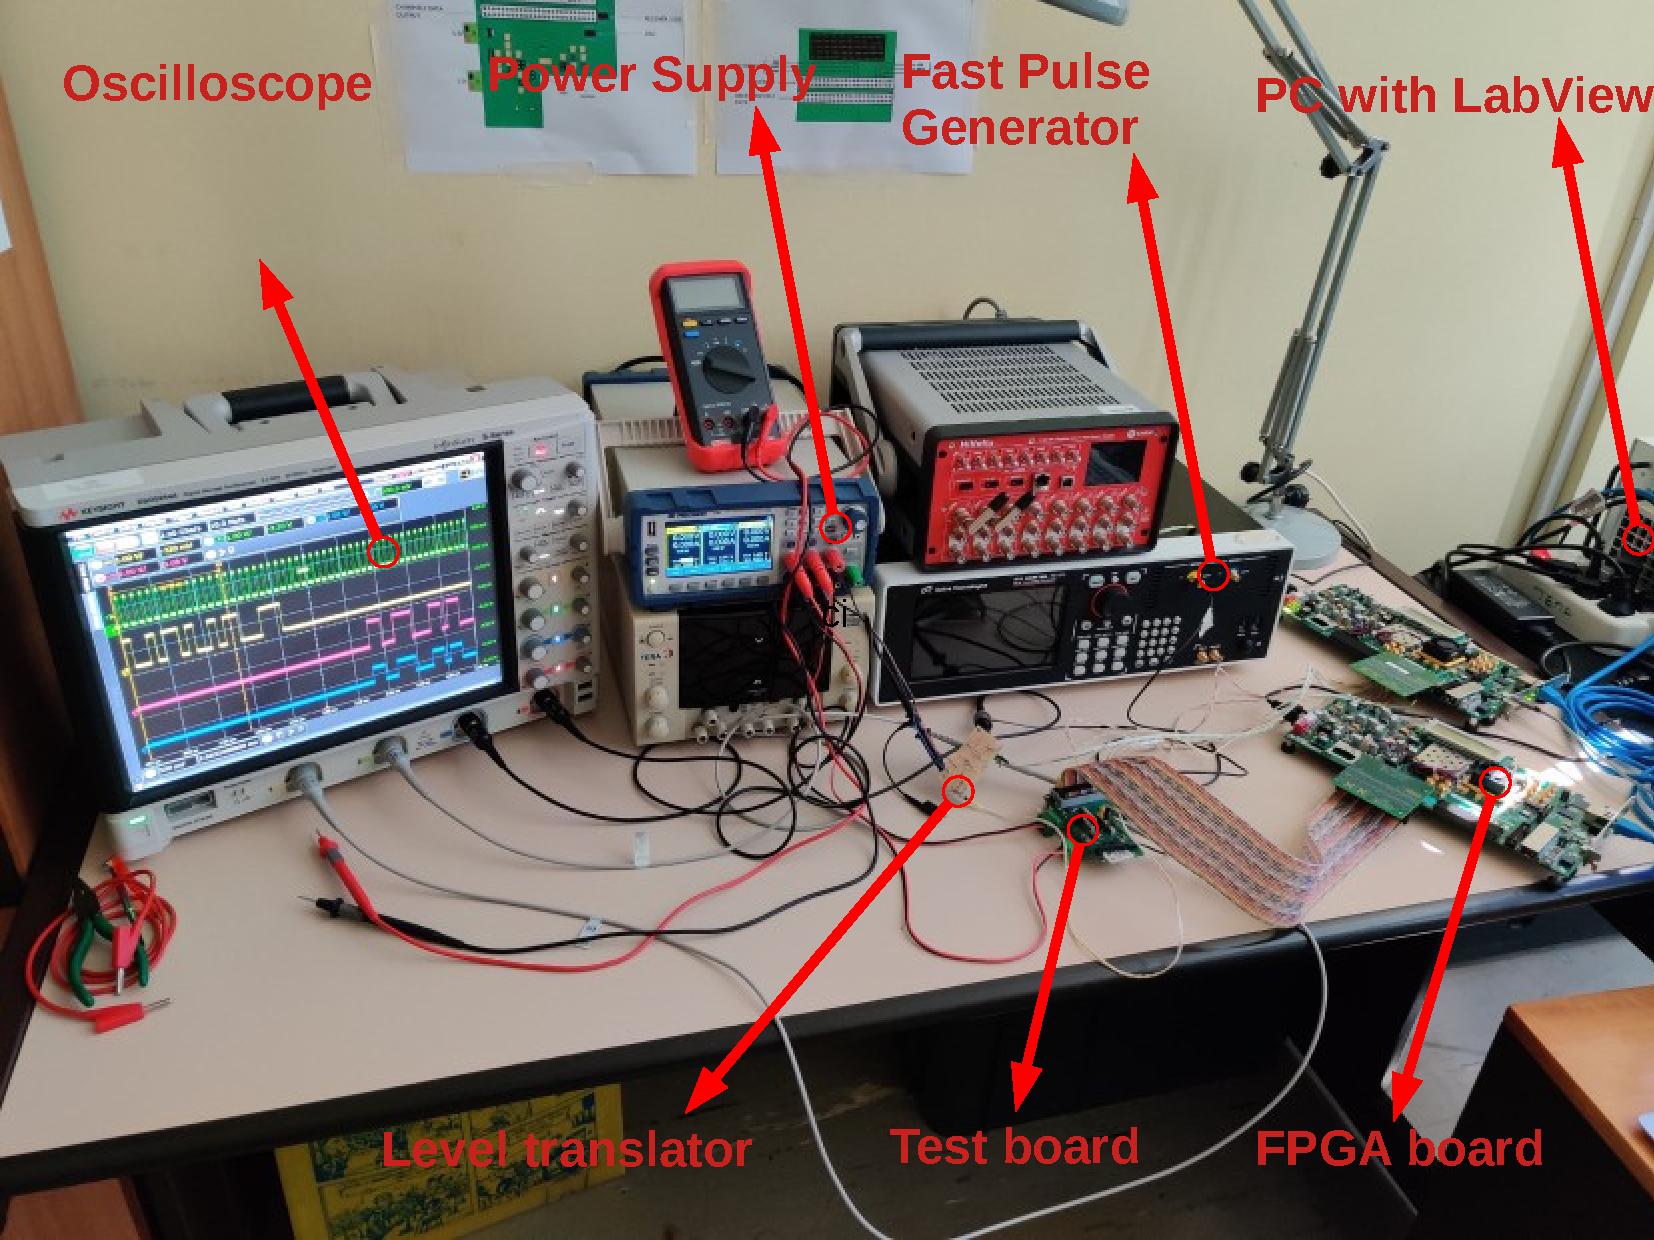
\includegraphics[width=0.7\linewidth]{IMG/ch5/TESTBENCH}
	\caption{Experimental setup and devices.}
	\label{fig:testbench}
\end{figure}
In order to properly validate the new additions to the FPGA firmware, after the simulations performed in the Vivado design suite, numerous tests have been carried out on the FPGA board and on chip.
The setup used to perform the tests is shown in figure \ref{fig:testbench} and it comprehends:
\begin{itemize}
	\item \textit{KEYSIGHT DSOS254A} (Digital Storage Oscilloscope), 4-channels, 2.5~GHz, 20~GSa/s, 10~bit ADC professional oscilloscope
	\item \textit{BK PRECISION 9140} power supply for the test board and the level translator device of section \ref{leveltranslator}
	\item \textit{ACTIVE TECHNOLOGIES} Fast Pulse Generator (70~ps Pulse/Delay) used to simulate the signal coming from the detector
	\item A computer with LabVIEW 
	\item The FPGA board with the firmware extensions to be tested
	\item The test board with the ABACUS2 bonded to it
	\item A level translator circuit required to boost the output data from the ABACUS2 I2C controller
\end{itemize}

\section{Test board}\label{testboard}
\begin{figure}[H]
	\centering
	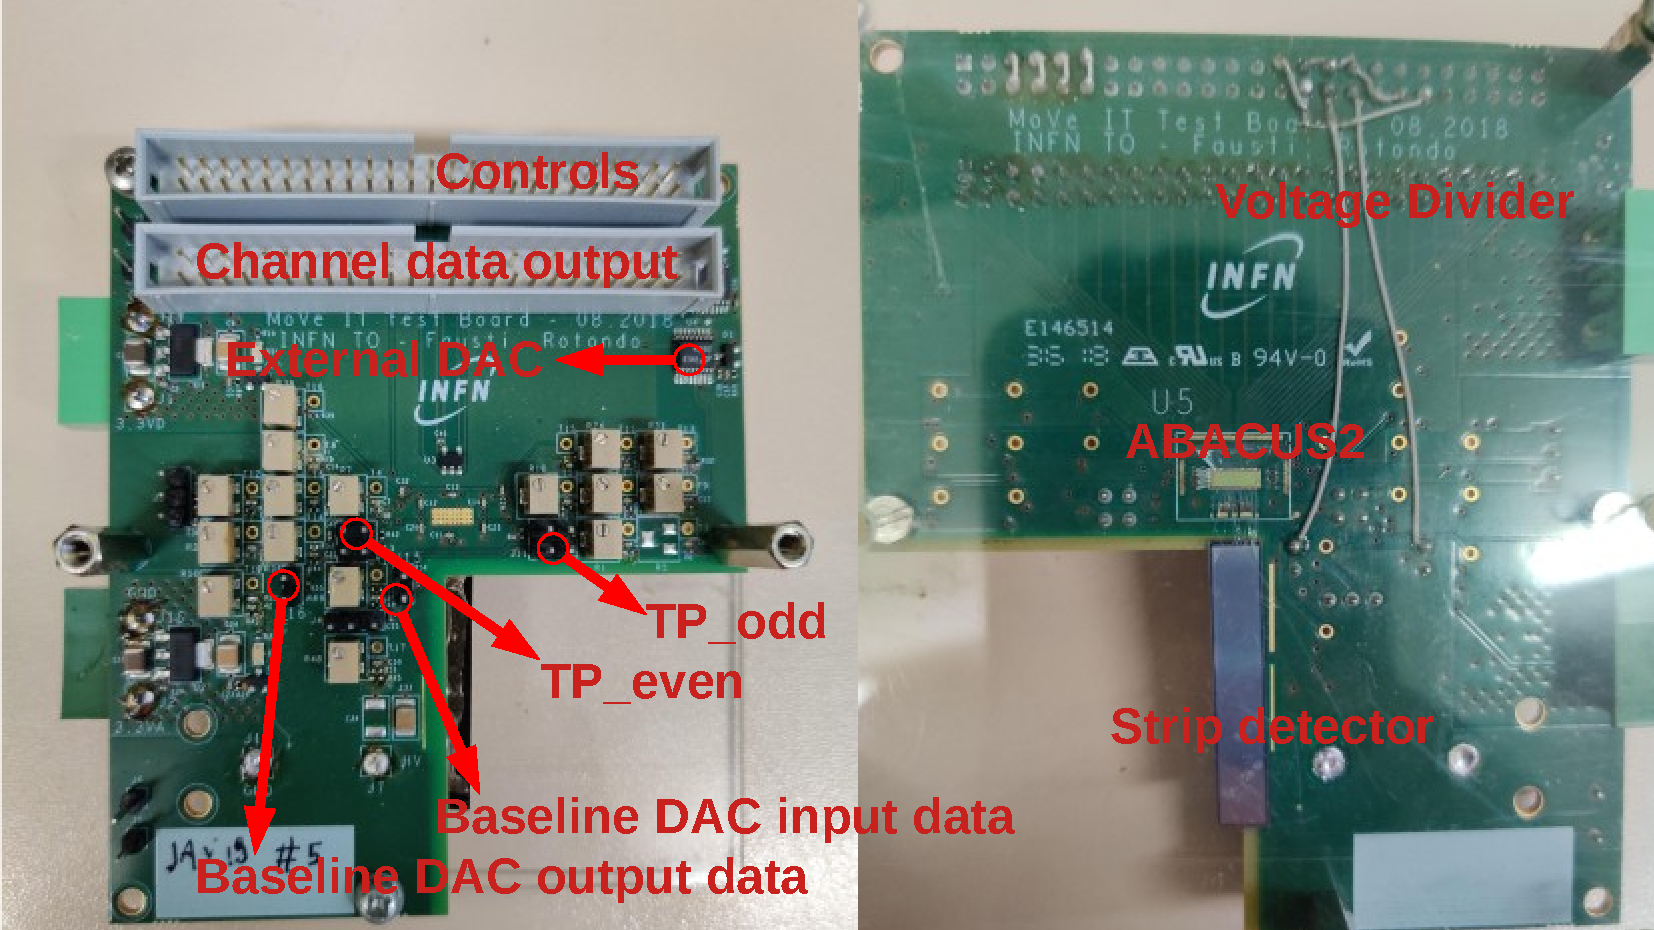
\includegraphics[width=0.9\linewidth]{IMG/ch5/TESTBOARD}
	\caption{Test board top and bottom view.}
	\label{fig:testboard}
\end{figure}
To test every feature of the ABACUS2 chip the INFN Turin section designed a custom test board.
On the back side of the PCB, shown in figure \ref{fig:testboard}, it can be observed the naked chip bonded to the board.
The main components of the test board are:
\begin{itemize}
	\item Two 50 pin connectors, the bottom one is used to send the differential data from the chip to the FPGA and the top one is used to transmit the controls (main DAC, trimming DACs, clocks) from the FPGA to the board;
	\begin{figure}[H]
		\centering
		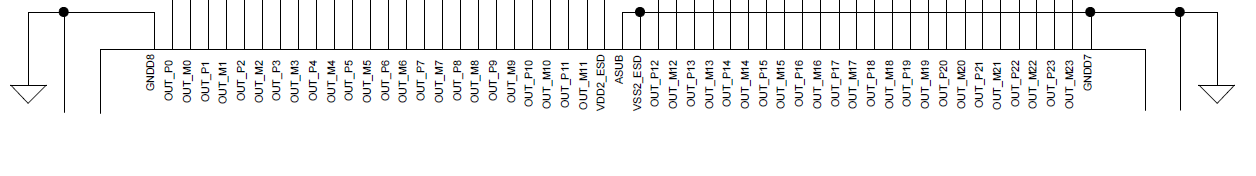
\includegraphics[width=0.95\linewidth]{IMG/ch5/DATATOFPGA}
		\caption{Wiring from the chip to the bottom 50 PIN connector.}
		\label{fig:datatofpga}
	\end{figure}
	\item The external DAC, a commercially available Linear Technology LTC2604 Quad 16-bit Rail-to-Rail DAC~\cite{LTC2604}, connected as in figure \ref{fig:externaldac};
	\begin{figure}[H]
		\centering
		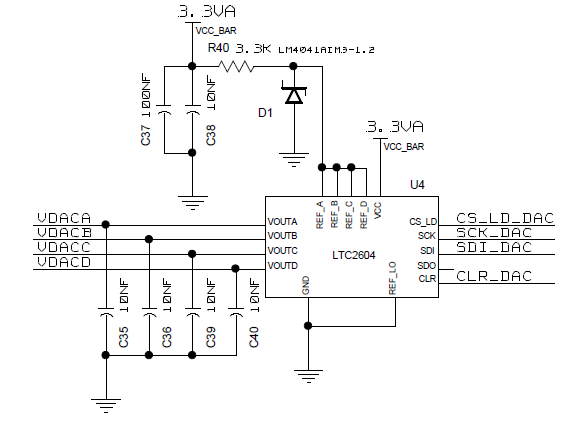
\includegraphics[width=0.3\linewidth]{IMG/ch5/EXTERNALDAC}
		\caption{Connections of the LTC2604 external DAC.}
		\label{fig:externaldac}
	\end{figure}
	\item Two TP (Test Pulse) connectors (\textit{TP\_odd} and \textit{TP\_even}) used to inject a charge respectively to the odd and even input channels of the chip, to emulate the signals form LGAD detectors (figure \ref{fig:tpconnector});
	\begin{figure}[H]
		\centering
		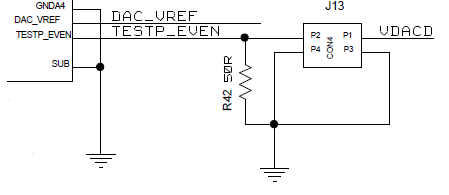
\includegraphics[width=0.4\linewidth]{IMG/ch5/TPCONNECTOR}
		\caption{Wiring of the \textit{TP\_even} connector.}
		\label{fig:tpconnector}
	\end{figure}
	\item Two connectors (Data INput and Data OUTput) used to send and receive data to and from the internal DACs, wired as in figure \ref{fig:internaldacwiring} with a 50~$\Omega$ termination.
	\begin{figure}[H]
		\centering
		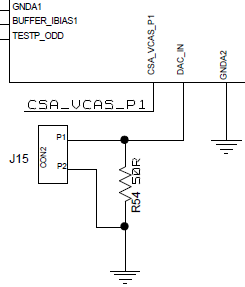
\includegraphics[width=0.2\linewidth]{IMG/ch5/INTERNALDACWIRING}
		\caption{Wiring of the Data INput (trimming/internal) DAC connector.}
		\label{fig:internaldacwiring}
	\end{figure} 
\end{itemize} 
\noindent The 50 PIN connector is connected to the FMC port by means of an additional custom breakout board that can be seen attached to the FPGA in figure \ref{fig:testbench}. This adapter PCB has no electrical components and only provides wiring to adapt one physical connector to another.
It has to be noted that the ABACUS2 test board has many trimmers and test pads.
These are used to regulate and measure different voltages of the chip. This is mandatory for a proper characterization of the ASIC.
\section{Hardware devices}\label{hardware}
\noindent As described previously, the configuration and readout of the internal DACs of the ABACUS2 chip works using 1.2~V LVCMOS single-ended signals.
However, since the FPGA uses only one reference voltage for the entire FMC connector, at 2.5~V, it is impossible to send and receive 1.2~V signals.
In order to solve this problem two simple circuits have been implemented: a voltage divider and a level translator device.
\subsection{Voltage divider}
The data coming from the FPGA to the chip are transmitted using serial protocols with 2.5~V single-ended signals.
To lower this value to 1.2~V two simple voltage dividers were implemented with 2 SMD (Surface-Mount Devices) and a 1/4~W ceramic resistor each on the back of the test board. This can be seen in figure \ref{fig:voltagedivider} and \ref{fig:testboard}.
\begin{figure}[H]
	\centering
	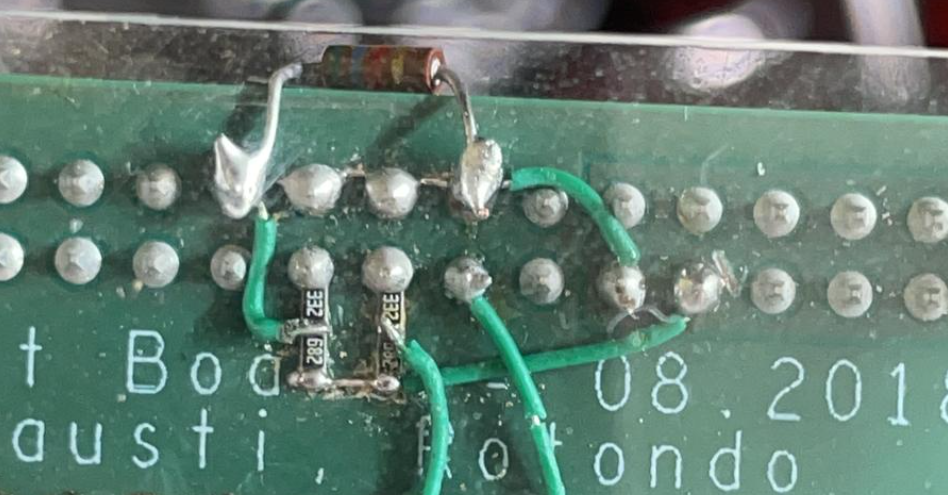
\includegraphics[width=0.6\linewidth]{IMG/ch5/VOLTAGEDIVIDER}
	\caption{Voltage dividers on the back of the test board, one is used for the clock signal and one for the data input.}
	\label{fig:voltagedivider}
\end{figure}
\noindent To obtain the 1.2~V output voltage three resistors were used: a 3.3~k$\Omega$ one for the first stage and a 6.8~k$\Omega$ and 5.6~k$\Omega$ placed in parallel for the second stage.
\subsection{Level translator}\label{leveltranslator}
The data coming from the ABACUS2 internal DACs I2C controller are 1.2~V CMOS. This value is too low and thus the board reads it as a logic \textit{low} value. A voltage translation circuit is mandatory in order to boost the signal \textit{high} value at 2.5~V, as expected from the FPGA.
\begin{figure}[H]
	\centering
	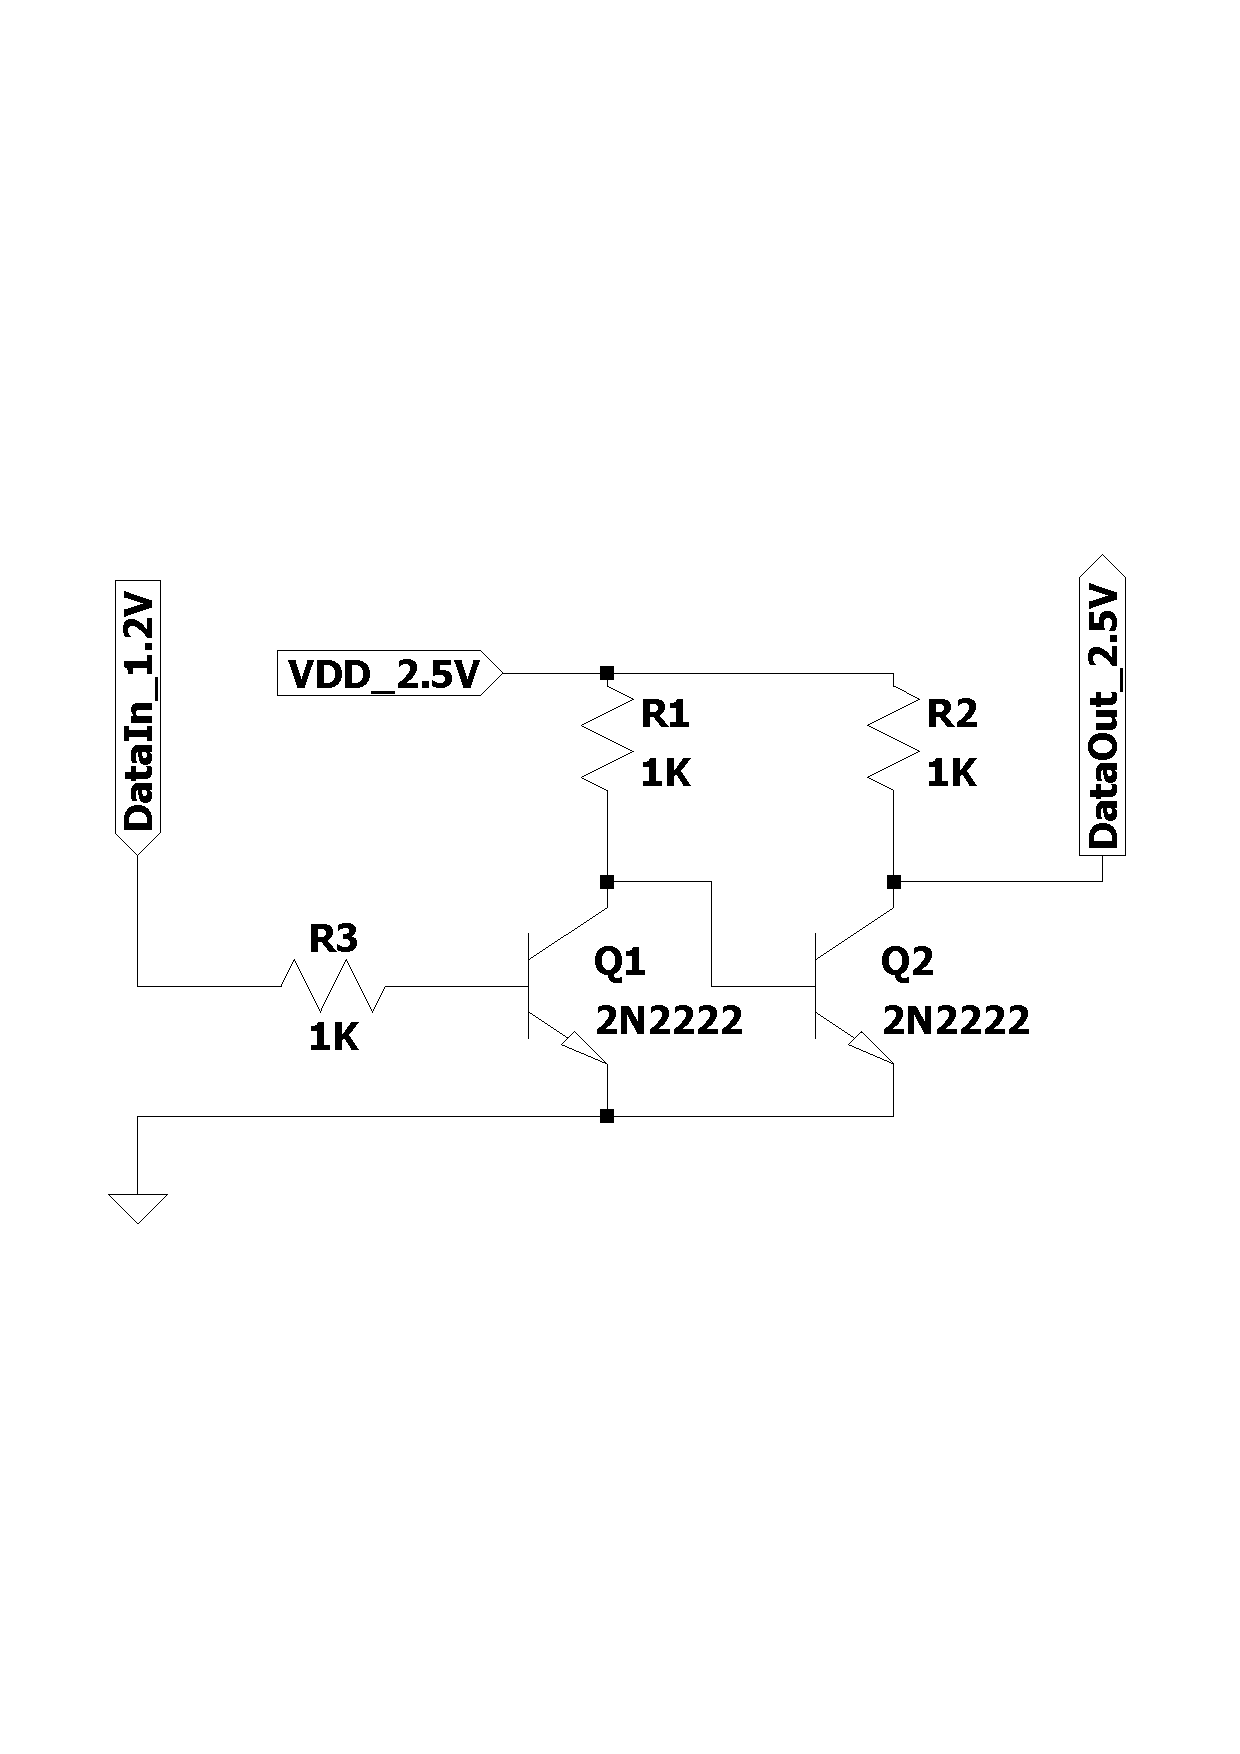
\includegraphics[width=0.6\linewidth]{IMG/ch5/DIAGRAM}
	\caption{Diagram of the level translation device.}
	\label{fig:diagram}
\end{figure}
\noindent For this purpose I created the simple circuit, with the schematics shown in figure \ref{fig:diagram}, using three 1~k$\Omega$ resistors and two classic \textit{2N2222} transistors that are configured in the standard common emitter mode.
This device has been simulated using the LTspice simulator and the results can be seen in figure \ref{fig:transsimulation}.
The green signal is the input data at 1.2~V while the purple one is the output signal at 2.5~V.
According to the simulation the device works properly and thus it was implemented in hardware.
\begin{figure}[H]
	\centering
	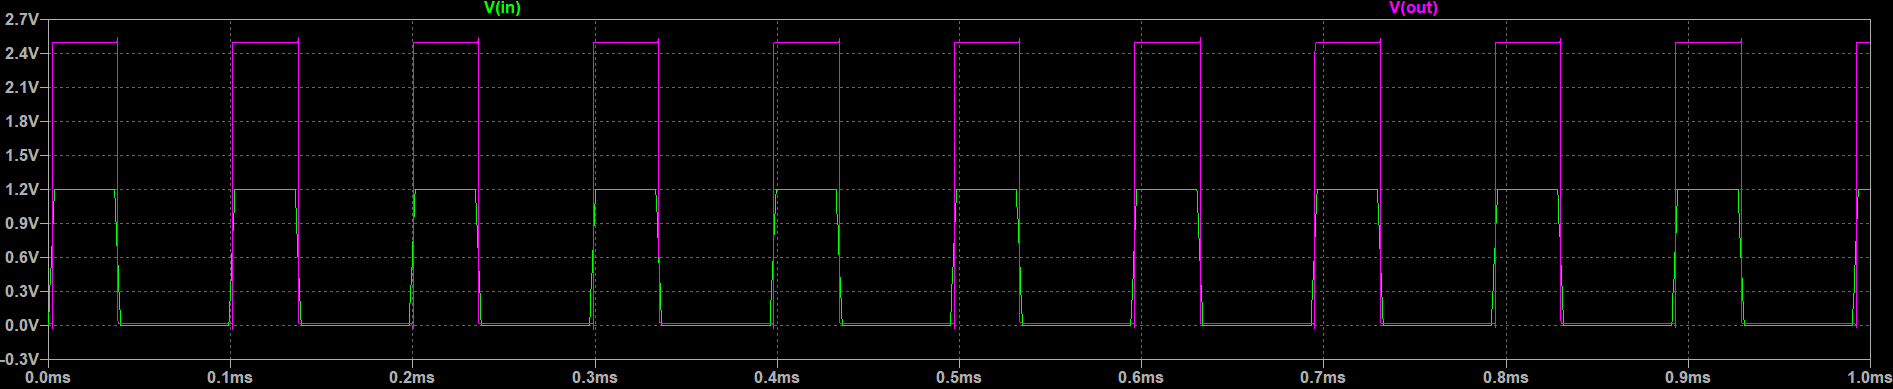
\includegraphics[width=1\linewidth]{IMG/ch5/TRANSSIMULATION}
	\caption{LTspice simulation of the translation device.}
	\label{fig:transsimulation}
\end{figure}
\noindent The device was built by soldering the components on a piece of perfboard as shown in figures \ref{fig:fronttranslator} and \ref{fig:backtranslator}.
It needs to be externally powered with 2.5~V; however, in order to assure the safety of the FPGA board, the voltage was set to 2.45~V and the current was limited to 0.05~A. 
\begin{figure}[H]
	\centering
	\begin{minipage}{.5\textwidth}
		\centering
		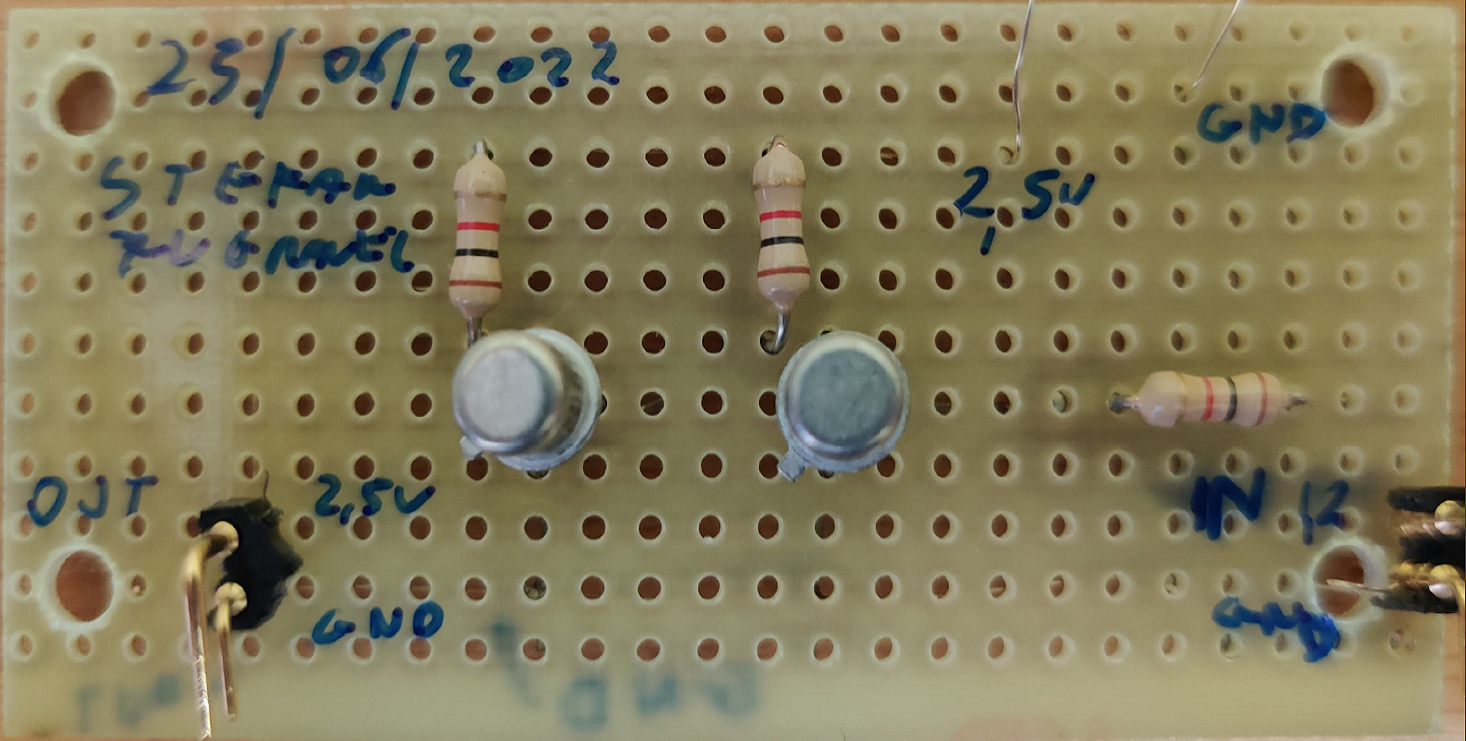
\includegraphics[width=.99\linewidth]{IMG/ch5/FRONTTRANSLATOR}
		\caption{Front view of the \\implemented translation device.}
		\label{fig:fronttranslator}
	\end{minipage}%
	\begin{minipage}{.5\textwidth}
		\centering
		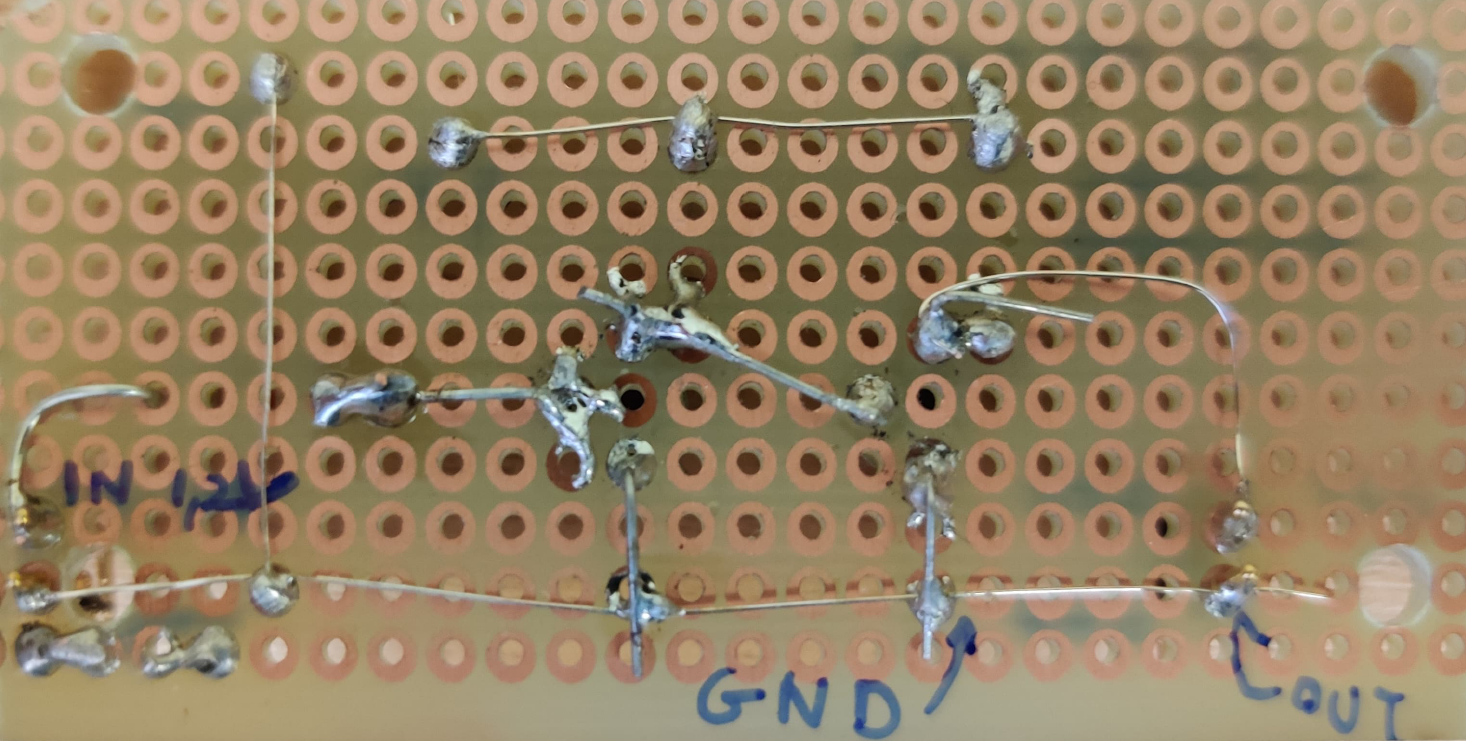
\includegraphics[width=.99\linewidth]{IMG/ch5/BACKTRANSLATOR}
		\caption{Back view of the \\implemented translation device.}
		\label{fig:backtranslator}
	\end{minipage}
\end{figure}

\section{Firmware validation on board}
The validation of the updated firmware was performed in two separate moments, the first one was done in May 2021 to test the trimming DACs, while the second one was carried out in October 2021 to validate the latch system and the timestamp generator. 
\subsection{Trimming DAC test}\label{dactests}
The trimming DAC validation process was divided into three parts, the verification of the clock period and the amplitude of the signal, the verification of the writing sequence and finally the verification of the reading process. 
All this tests were performed with the FPGA connected to the ABACUS2 test board and the relevant signals were probed with the oscilloscope. The test board was powered with two 3.3~V rails (analog and digital devices are powered independently).
\subsubsection{Clock and amplitude}
For this first part the goal was to validate the clock period and its amplitude. In order to do that a write non-specified command was sent while probing the \textit{baseline\_dac\_sck} signal. 
\begin{figure}[H]
	\centering
	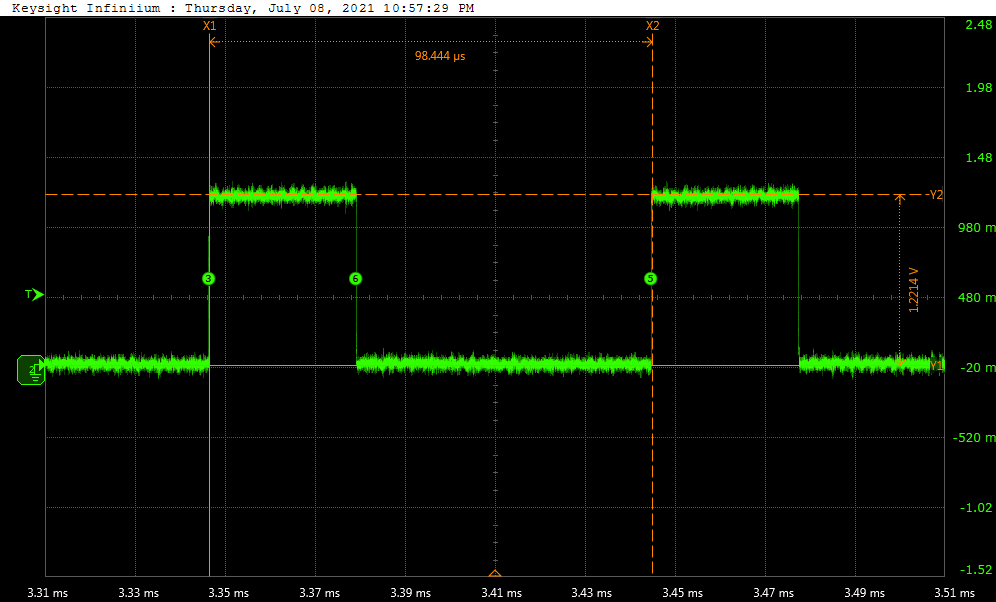
\includegraphics[width=0.7\linewidth]{IMG/ch5/probe/09-08-2021_clock-specks}
	\caption{\textit{baseline\_dac\_sck}; period and amplitude measurements.}
	\label{fig:clockspecs}
\end{figure}
\noindent In section \ref{confing} it was underlined that the clock period should theoretically be 98.28~$\mu$s, in figure \ref{fig:clockspecs} it can be seen that the measured period is 98.44~$\mu$s. The difference between the two periods is 160~ns, corresponding to about $\approx$0.16\% of the total. The period can be then considered perfectly compatible.
The second value to be noted in figure \ref{fig:clockspecs} is the amplitude of the signal, which is 1.22~V, perfectly safe for the chip. 

\subsubsection{Write sequence}
\noindent In order to write into the trimming DACs and to read from them, a new LabVIEW panel was implemented~\cite{data}. This piece of software, with the graphical interface shown in figure \ref{fig:labview3}, sends and receives the commands discussed in section \ref{InternalDac}. In addition it implements some useful features like:
\begin{itemize}
	\item the ability to write on only one DAC at a time with the \textit{Set Internal DAC} button
	\item the ability to write every DAC with a single \textit{Set multiple internal DAC} button press
	\item the possibility to read only one DAC value at the time with the \textit{Read ONE Internal DAC} button
	\item the possibility to read every DAC with a single \textit{Read Internal DACs} button press
	\item the ability to chose for each DAC channel if the signal needs to be sent to the HPC or LPC FMC
\end{itemize}
\begin{figure}[H]
	\centering
	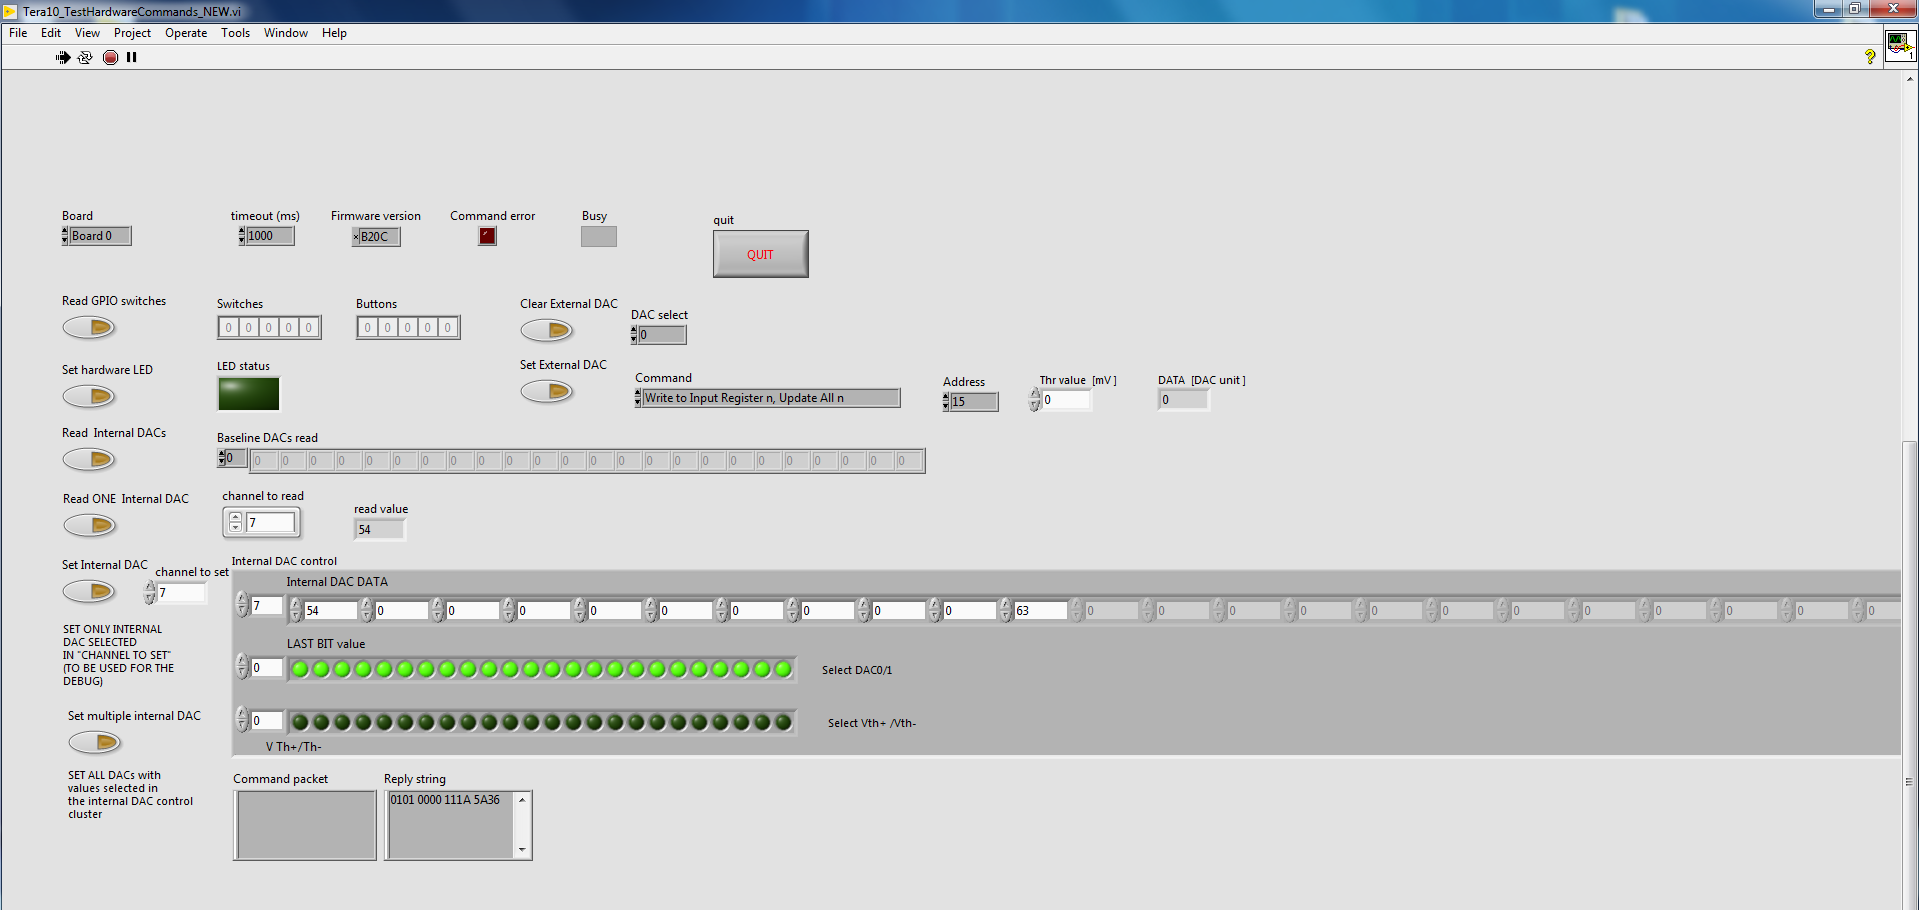
\includegraphics[width=0.99\linewidth]{IMG/ch3/LABVIEW2}
	\caption{LabVIEW tool coded by \textit{Emanuele Data} for the configuration of the trimming DACs.}
	\label{fig:labview3}
\end{figure}
\begin{figure}[H]
	\centering
	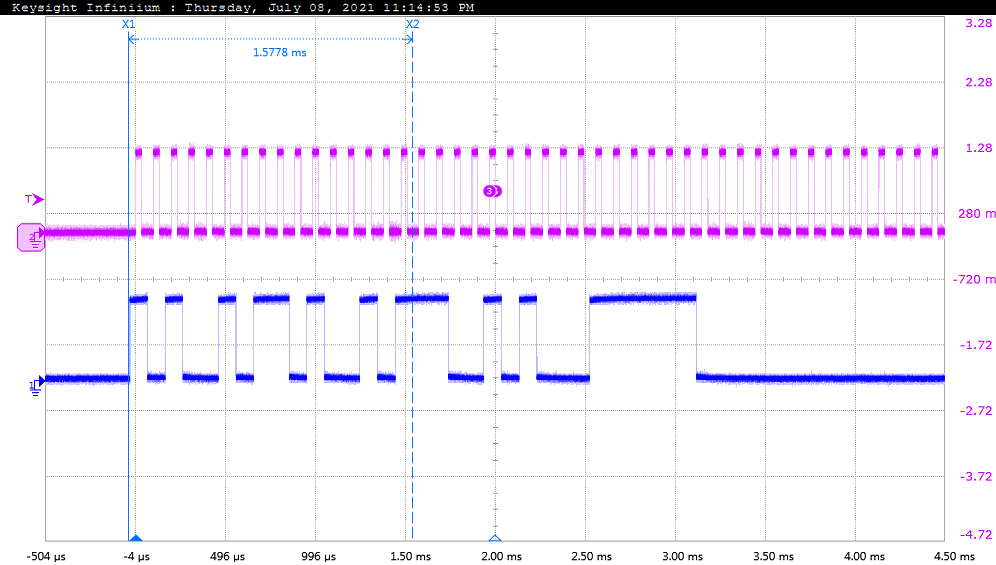
\includegraphics[width=0.7\linewidth]{IMG/ch5/probe/09-08-2021_ch05-write63-baselinedac1}
	\caption{Writing sequence, channel 5, word 63, DAC 1\\{\color{magenta}purple}= clock, {\color{blue}blue}= data out.}
	\label{fig:ch05write63}
\end{figure}
\noindent In figure \ref{fig:ch05write63} an example reading sequence being sent to the chip from an oscilloscope snapshot is shown.
The purple signal is the clock discussed previously while the blue one corresponds to the serial data being sent to the DAC controller.
Time scale is 0.5~ms/division, while vertical scale is 1~V (the signals were probed after the voltage divider). 
The two vertical markers delimit the initialization sequence, which is \textit{0xA5A5}~=~\textit{0b1010-0101-1010-0101}.
After the initialization, the two command bit sequence follows, in this case (Writing) they are \textit{0b11}.
Next in the sequence there is the 6~bit channel address which is divided into a 5~bit address plus a 1~bit V$_{th}$ selector.
This last bit is not used for the tested chip version, thus it was always set to zero (\textit{low}).
The remaining 5~bits are \textit{0d5}~=~\textit{0b0-0101} thus channel 5. The remaining 8~bits are divided into 2 unused bits (the MSB) and 6 data bits.
In this case these bits are \textit{0d63}~=~\textit{0b0011-1111}, the maximum possible value for a 6~bit DAC.
After the clock continues for 16 more cycles while the data line stays \textit{low}.
For the moment the user has no way of knowing if the chip was properly configured because it does not send any feedback while writing. In order to verify if the DACs are properly configured a reading procedure needs to be carried out. This will be analyzed in the next subsection.  

\subsubsection{Read command}
\begin{figure}[H]
	\centering
	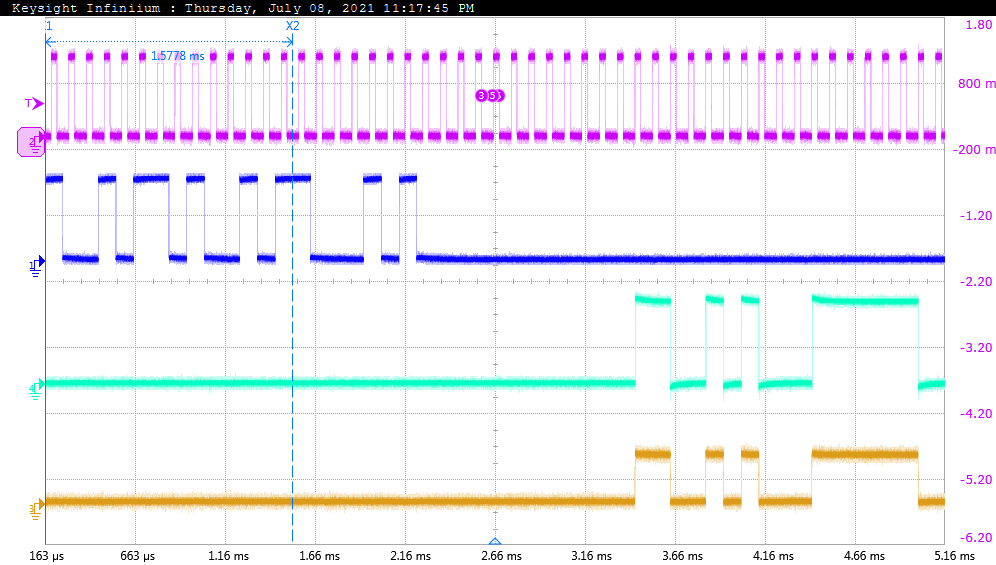
\includegraphics[width=0.7\linewidth]{IMG/ch5/probe/09-08-2021_ch05-read63-baselinedac1}
	\caption{Reading sequence, channel 5, word 63, DAC 1\\{\color{magenta}purple}= clock, {\color{blue}blue}= data out,\\{\color{cyan}cyan}= data in, {\color{orange}orange}= data from chip.}
	\label{fig:ch05read63}
\end{figure}
\noindent Figure \ref{fig:ch05read63} shows an oscilloscope snapshot with the reading sequence being performed on the same channel as before (\textit{ch05}).
The purple signal corresponds to the clock, the blue one to the serial data sent to the chip, the orange one to the data going from the chip to the level translator and in cyan there is the data from the level translator to the FPGA.
Division is 0.5~ms wide, while each vertical division corresponds to 1~V for the green and yellow signals and 2~V for the red and blue signals.
Between the two markers there is the initialization sequence \textit{0xA5A5}~=~\textit{0b1010-0101-1010-0101}, followed by the 2-bit read command \textit{0b10} and by the address to be read, in this case channel 5, thus \textit{0d5}~=~\textit{0b0-0101} as before.
When sending a read command, the 8~bit data are not considered and the firmware drives them \textit{low}.
The output from the chip is 1.2~V, too low to be read by the board, for this reason the signal is boosted by the level translator up to 2.5~V (in cyan).
The data sent by the chip is made up by 16~bit words. The first 2~bit are a \textit{"read confirmation"} signal 0b11. The next 6 bit are the confirmation of the selected channel, in this case \textit{0d5}~=~\textit{0b0-0101} plus \textit{0b0} for the V$_{th}$ selector.
The chip is reading from the same channel that was configured before.
The last 8~bit are the read value, in this case \textit{0d63}~=~\textit{0b0011-1111}.
The read value is the same as the configured one. This means that the firmware and the chip are working properly.
It is interesting to consider that the trimming DACs do not retain their state.
When the chip is powered off after the configuration, the DACs settings are lost and at the next power on the DACs will start from their initial values.
It is important to know that this initial value is not always zero, but some random value due to the manufacturing process.
This behaviour makes the ability to read and configure these DACs even more important for every data taking. In appendix \ref{DacAppendix} there are more examples of write and read sequences. 
\subsubsection{Threshold scan}\label{considerations}
%%%%%%%%%%%%%%%%%%%%%%%%%%%%%%%%%%%%%%%%%%%%%%%%%%%%%%%%%%
\begin{figure}[H]
	\centering
	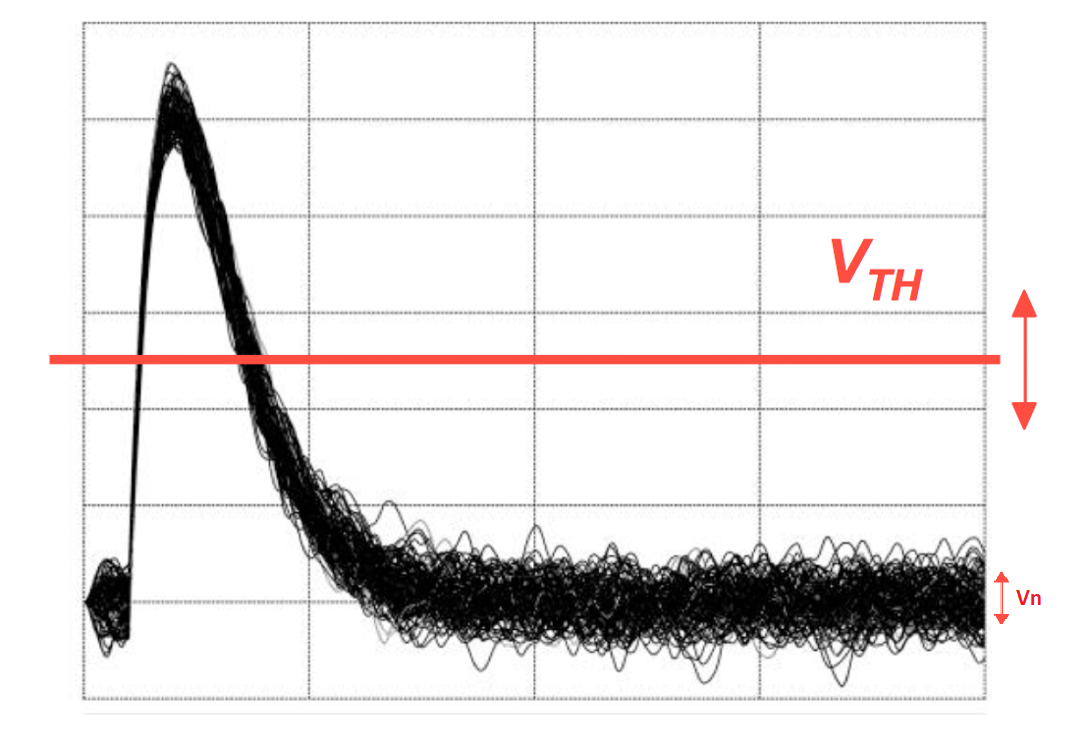
\includegraphics[width=0.7\linewidth]{IMG/ch5/DataDacConfig/tscan_sketch2}
	\caption{Threshold scan example~\cite{rivetti}.}
	\label{fig:tscansketch}
\end{figure}
\noindent The ABACUS2 chip implements a binary readout system. As a consequence, any signal crossing the threshold ($V_{th}$) is processed as a good event~\cite{rivetti}.
Therefore, it is important to minimize the number of hits due to noise, which requires a proper setting of the comparator threshold. It can be proven that the frequency of noisy hits can be estimated as
\begin{equation}
	f_n=\frac{1}{4 \sqrt{3} \tau} e^{- \frac{V^2_{th}}{2V^2_n}} 
\end{equation}
\noindent where $f_n$ is the number of noisy hits per second, while V$_{th}$ is the applied threshold voltage measured from the front-end amplifier baseline and $V_{n}$ is the RMS noise voltage measured at the front-end amplifier output.
For example, a time constant $\tau$ of 50~ns and a threshold-to-noise ratio of 4 lead to 968 noisy hits per second in one channel.
This number drops to $5.5\cdot10^{-16}$ if the threshold-to-noise ratio is 10, to be compared to the number of expected hits in a strip at the nominal working flux of several MHz.
As a rule of thumb, a signal-to noise ratio of between 10 and 15 on the minimum signal of interest allows to work with thresholds high enough to suppress almost completely the noise while preserving a good efficiency.
A binary system, such as the ABACUS2 chip, is usually tested with the method of the “S-curve”.
The probability that a signal with a given average amplitude exceeds
the threshold can be calculated as follows:
\begin{equation}
	P(V>V_{TH}) = \frac{1}{\sqrt{2\pi}\sigma} \int_{V_{TH}}^{\infty} e^{- \frac{(V-\mu)^2}{2\sigma^2}} dV
\end{equation}
The number of times the comparator fires is counted and the efficiency $\eta$
is calculated as:
\begin{equation}
	\eta = \frac{Number \: of \: detected \: signals}{Number \: of \: sent \: signals}
\end{equation}
The data can be thus fitted with a sigmoid function:
\begin{equation}\label{erf}
	\eta (V) = \frac{1}{2} [erf(\frac{V-\mu}{\sqrt{2}\sigma})+1]
\end{equation}
being:
\begin{equation}
	erf(x) = \frac{2}{\sqrt{\pi}} \int_{0}^{x} e^{-t^2} dt
\end{equation}
The point $\eta$ = 0.5 corresponds to input signals generating an output whose average is identical to the threshold. The parameters $\mu$ and $\sigma$ need to be extracted from the fit.
\begin{figure}[H]
	\centering
	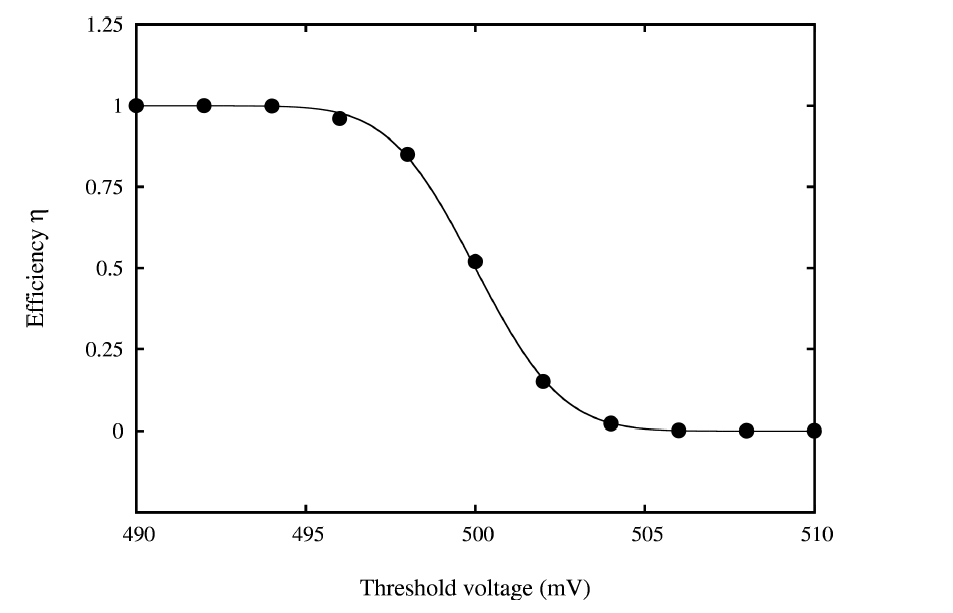
\includegraphics[width=0.65\linewidth]{IMG/ch5/THexample}
	\caption{Example of “S-curve” obtained by scanning the threshold voltage at fixed signal amplitude.}
	\label{fig:thexample}
\end{figure}
%%%%%%%%%%%%%%%%%%%%%%%%%%%%%%%%%%%%%%%%%%%%%%%%%%%%%%%%%%
\noindent The signal coming from the CSA (Charge Sensitive Amplifier) is a sum of two components, one in DC, that is referred to as "pedestal" and the signal that is being amplified.
As explained before, the chip sends a logic signal each time the output of the CSA is greater than a selected threshold value.
If the threshold voltage is less than the pedestal, the output of the chip will be always \textit{low}, thus the measured rate will be zero.
If the V$_{th}$ is approximately equal to the pedestal the chip will sample noise and the rate will explode.
When the V$_{th}$ is greater than the pedestal the chip is sampling only signal, as shown in figure \ref{fig:tscansketch}.
Incrementing even more the threshold voltage will cause a gradual death of the rate, the smoothness of the death is due to the noise.
If the signal were noiseless, the result of the threshold scan would be a reverse step function.
This decrease in the rate can be fitted with the error function defined in equation \ref{erf} to extract the siganl level and the $\sigma$ due to the noise.
\newline
\noindent This behaviour can be observed in figure \ref{fig:thscanch0}; the blue line is a threshold scan curve with trimming DAC fixed at \textit{0x00}~=~\textit{0d00} and variable external DAC, while the green corresponds to the same threshold scan but with trimming DACs configured at \textit{0x3F}~=~\textit{0d63}.
The measurements were performed with the fast pulse generator setted at 600~mV (injected charge =~24~fC) at 10~KHz on the odd channels. The data were extracted from ch1.
In figure \ref{fig:thscanch0} it can be observed the same behaviour described before.
At first, for low V$_{th}$, the rate is zero, when V$_{th}$ reaches the noise the counts explode and after this noise region the chip samples only signal, in this case at exactly 10~KHz.
Lastly the signal smoothly dies. 
By fitting the last part of the threshold scan with an error function it is possible to determine the output voltage of the amplifier corresponding to a given input charge.
By repeating this measurement for different input charges and extrapolating to zero input charge it is possible to determine the pedestal of the amplifier.
This measurements depend on the level of the DAC threshold.
\noindent The most important thing to observe in figure \ref{fig:thscanch0} is that a change of the trimming DAC value leads to a translation of the threshold scan curve, thus validating the configuration of the trimming DACs.
This translations is approximately 20~mV.
\begin{figure}[H]
	\centering
	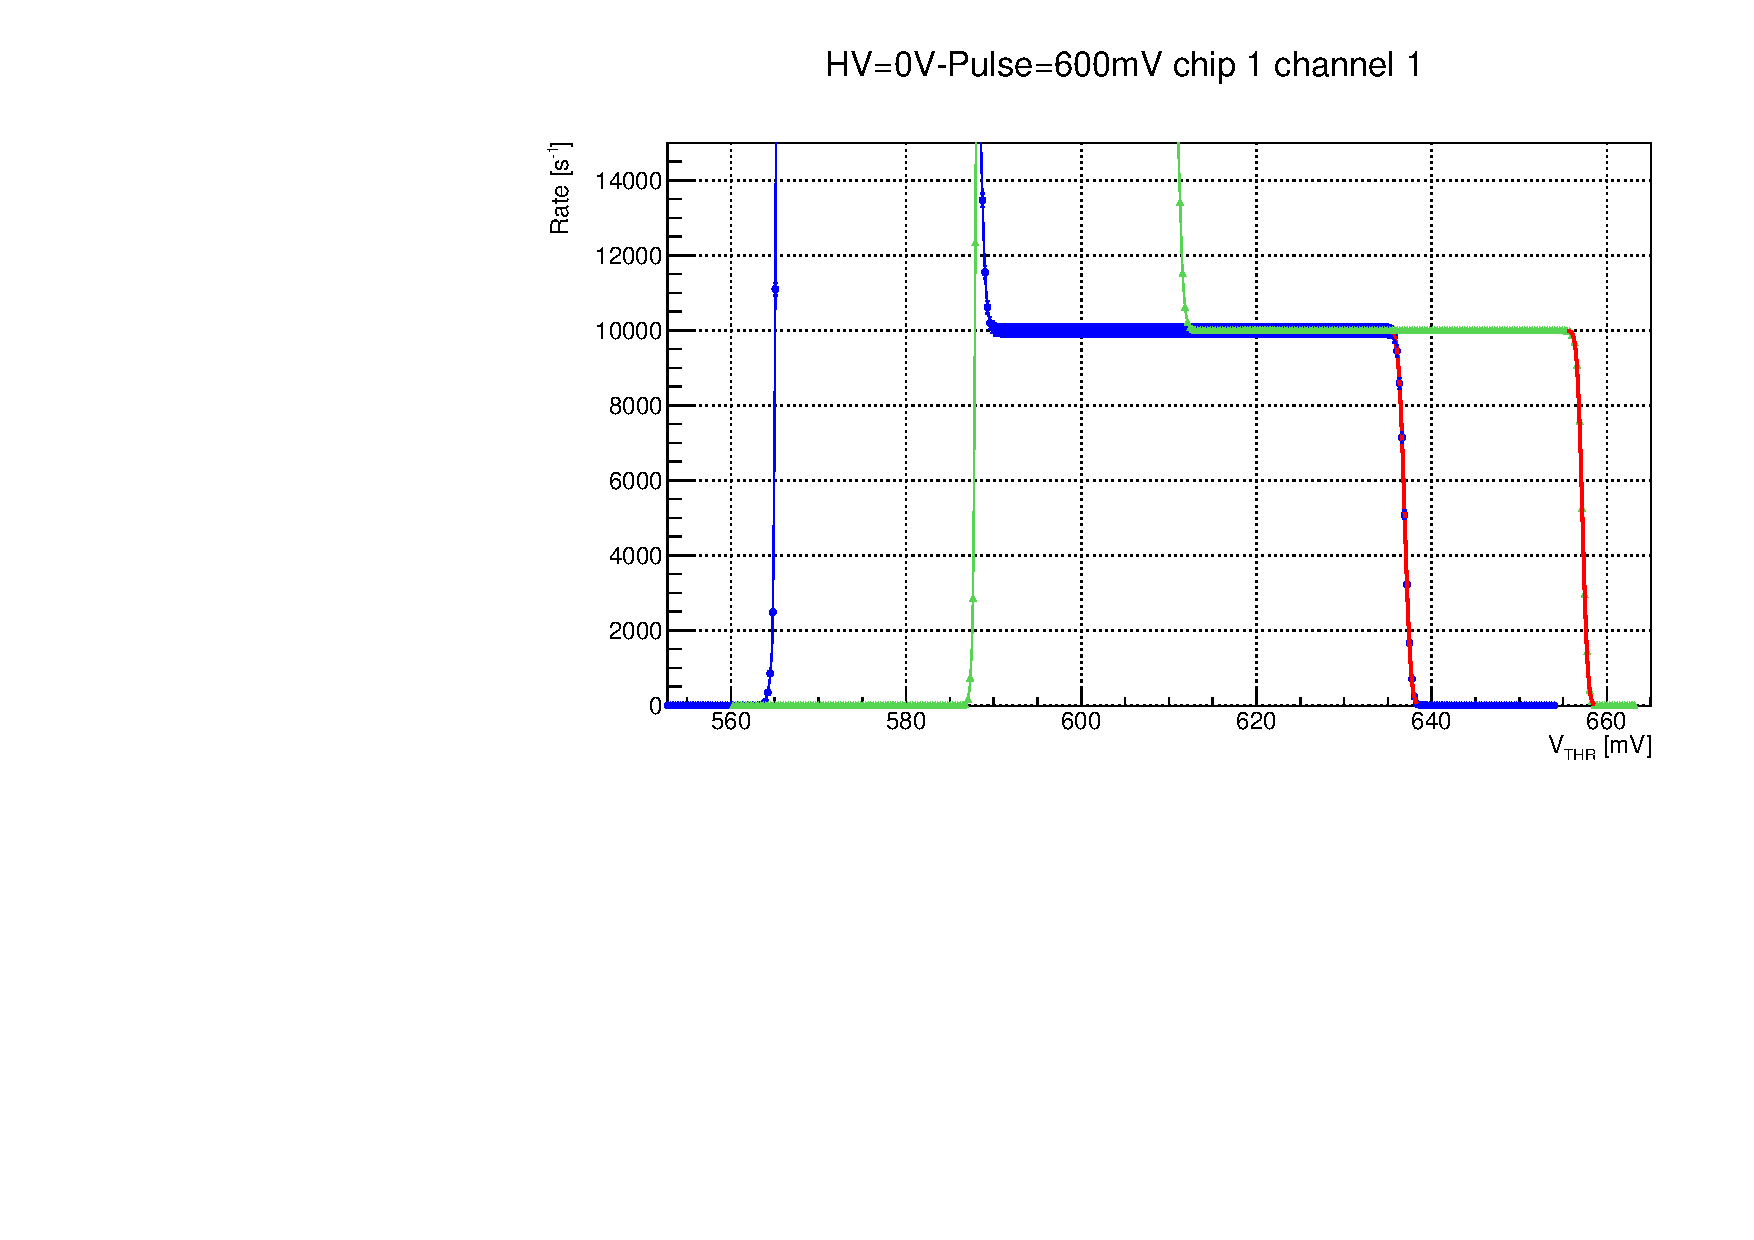
\includegraphics[width=0.8\linewidth]{IMG/ch5/DataDacConfig/ThScan_ch0.pdf}
	\caption{Sample S-curves obtained with: {\color{blue}blue}= trimming DAC at \textit{0d00},\\{\color{green}green}= trimming DAC at \textit{0d63}.}
	\label{fig:thscanch0}
\end{figure}

\begin{figure}[H]
	\centering
	\includegraphics[width=0.8\linewidth]{IMG/ch5/DataDacConfig/DAC_V_REF_600mv-Copia.pdf}
	\caption{{\color{blue}blue}= pedestal values with trimming DAC at \textit{0d00}, {\color{green}green}= pedestal values with trimming DAC at \textit{0d63}.}
	\label{fig:pedestal}
\end{figure}
\noindent After fitting the S-curves with the error function and calculating the pedestal voltages some more consideration can be taken.
In figure \ref{fig:pedestal} is can be seen a distribution of the pedestal voltages for some channels with trimming DAC configured at \textit{0d00} (blue) and at \textit{0d63} (green).
The average difference between the two values for each channel is approximately 20.9~mV.
In conclusion, the ability to change the trimming DACs values allows to reduce the differences in the DC output of the chip channels and thus to obtain a more accurate measurement of the particles rate.
%\newpage
\subsection{Latching counters test}\label{latchtests}
This section describes the verification of the main features of the new \textit{tera10\_latch\_counter} module.
This validation process, as well as the next one, was performed in a short period of time. This means that the new software, created for test purposes only, will not be the same used for future measurements.
It has to be noted that this firmware extensions do not change at all the Input/Output assignments of the board, the only difference is in how the data is being treated; in this case saved into a memory.
In order to test the new \textit{tera10\_latch\_counter} module a new LabVIEW panel (in figure \ref{fig:newlabviewpanel}) was designed by me and INFN researchers.
\begin{figure}[H]
	\centering
	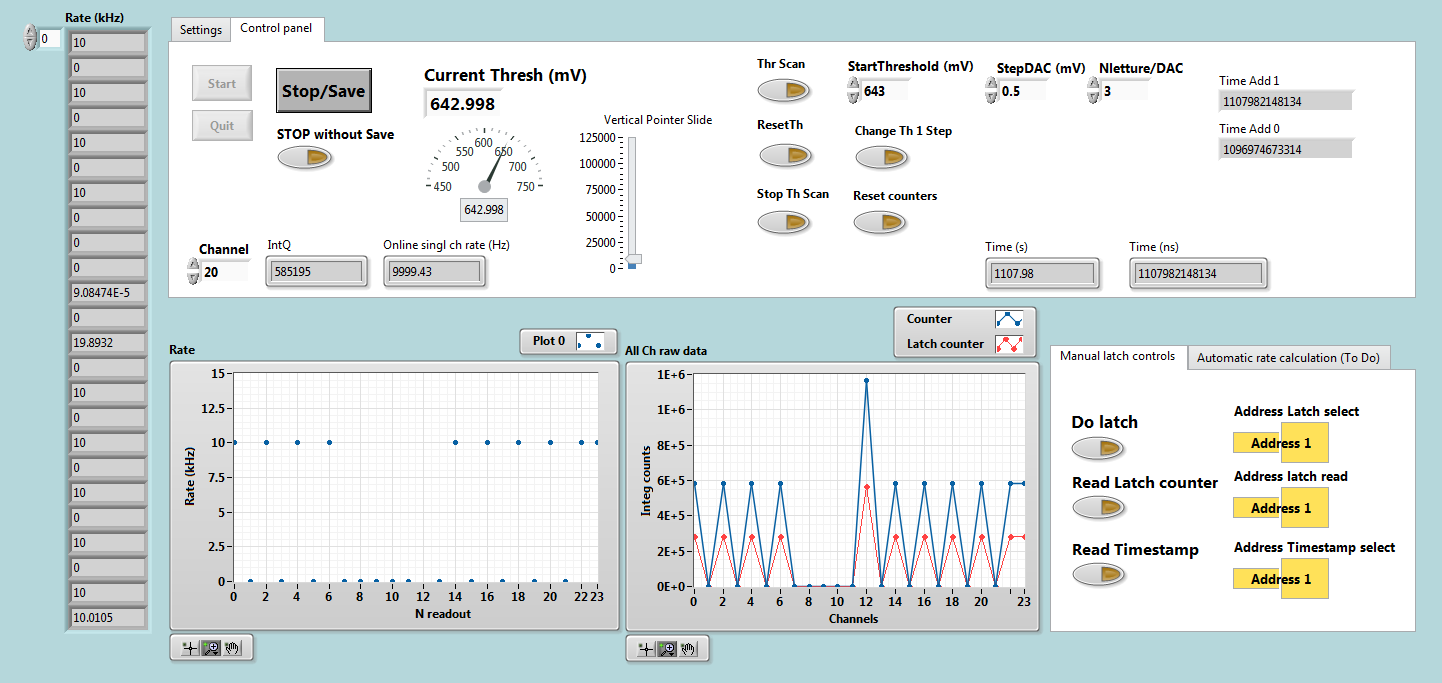
\includegraphics[width=0.99\linewidth]{IMG/ch5/latch_tests/fig1.PNG}
	\caption{New LabVIEW data acquisition panel used for rate measurements.}
	\label{fig:newlabviewpanel}
\end{figure}
\noindent This new piece of software allows new types of measurements that could not be performed before.
The first two commands tested were: \textit{do\_latch} and \textit{read\_latch\_counter}. The starting point was the already existing \textit{Tera10\_data\_acquisition\_panel}. This LabVIEW piece of software was programmed in such a way to give the user a "real time" reading of every counter [Online singl ch rate (Hz)].
This means that every time the software is running it sends to the FPGA some command that can be: configure a DAC, read a channel, reset, enable or disable selected channels.
When the \textit{DO LATCH} button is pressed a flag is raised, the LabVIEW logic sends the latching command and when it receives the response it goes back to the main state.
In figure \ref{fig:newlabviewpanel} it can be noted that there are two buttons, one for latching and one for reading the counters. For each button there is a boolean controller that allows the selection between address \textit{0} and \textit{1}.
By combining the reading and latching addresses four possibilities emerge:
\begin{itemize}
	\item \textbf{LATCH~=~0} and \textbf{READ~=~0 $\rightarrow$} every time the \textit{do\_latch} button is pressed and then the reading command is sent, the values displayed are being updated. The user is reading the latest saved latched values.
	\item \textbf{LATCH~=~1} and \textbf{READ~=~0 $\rightarrow$} this time the data is being saved on address \textit{1}, however we are still reading from address \textit{0}, this means that the data on the screen should stay the same as the case before.
	\item \textbf{LATCH~=~0} and \textbf{READ~=~1 $\rightarrow$} with this combination at the first reading command the read data value change, however this happens only the first time. Now the user is writing on address \textit{0}, but reading from address \textit{1}. 
	\item \textbf{LATCH~=~1} and \textbf{READ~=~1 $\rightarrow$} this case works as the first one, the user is reading from the same channel on which he is writing thus the data is always updated. 
\end{itemize}
\noindent By doing these four simple tests it turns out that the address system works as intended. The next step is to set the fast pulse generator to a known rate and to measure it using the new and improved latch system.
\begin{figure}[H]
	\centering
	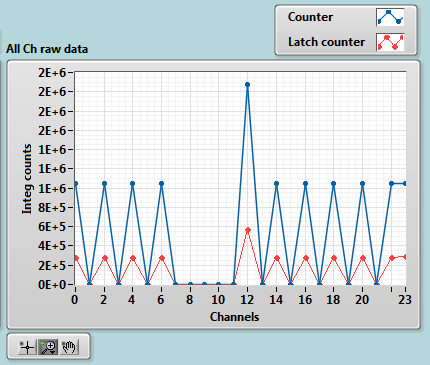
\includegraphics[width=0.5\linewidth]{IMG/ch5/latch_tests/fig2.PNG}
	\caption{Latch counter measurement on graph.}
	\label{fig:latchfigure}
\end{figure}
\noindent In figure \ref{fig:latchfigure} it can be seen the behaviour of the latch system. On the X axis there is the channel number and on the Y axis there is the total number of counts; the test pulses are being sent only to even channels, however it can be seen that not every channel is counting and others, for example \textit{ch23}, are suffering from cross talk problems. Some other channels, like \textit{ch12}, have counts almost doubled. This is known as "counting for after pulse" and happens when the threshold value is not perfectly setted and some noise is being counted.
The key point in this figure is the red line. This is the last read latch value.
When pressing the \textit{Do latch} button the "blue dots" value is saved into the FPGA, when reading the latch this data appears on the graph as "red dots".
These last points are fixed, they do not move if the user does not sends another \textit{Do latch} and \textit{Read Latch counter} command. However, the blue line gradually rises.
This means that doing a latch is like taking a photo of a bunch of moving gauges, it instantly fixes they value without stopping them.  
\subsection{Timestamp generator test}
\noindent As explained in chapter 4, the timestamp generator is a 64~bit counter that can be read in four 16~bit sections.
I updated the LabVIEW data acquisition panel in order to implement the \textit{read\_timestamp} command.
The final LabVIEW piece of software, that can be seen in figure \ref{fig:newlabviewpanel}, has a button to read the timestamp and a boolean controller to select the address.
The read value is shown as an integer in indicators \textit{Time add 1} and \textit{Time add 2}. The last read timestamp is also converted in nanoseconds~(\textit{ns}) and in seconds~(\textit{s}).
To be noted that the timestamp can not be restarted, it starts from zero when the board turns on and always counts, thus the \textit{Time~(s)} could also be a "\textit{Wake time}" indicator. A reset command was not implemented because not necessary. The timestamp is used only for time differences and, since it could stay on for 1000~years without restarting, there is no need for a reset button. 
These values can be seen in figure \ref{fig:timestampfigure}
\begin{figure}[H]
	\centering
	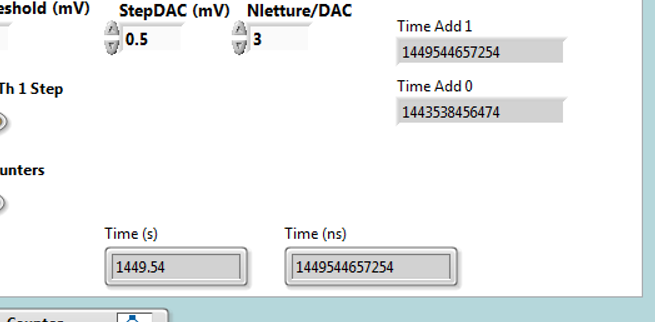
\includegraphics[width=0.5\linewidth]{IMG/ch5/latch_tests/fig15.PNG}
	\caption{Details of the Timestamp indicators values. For example in this case the timestamp measurement was done $\approx$~24~min after the board was turned on.}
	\label{fig:timestampfigure}
\end{figure}
\noindent A proper performance test of this new feature is presented in the next subsection. However, a simple measurement was performed in order to check if the timestamp counter runs at a "reasonable speed".
This was done simply by saving the timestamp data and starting a chronometer at the same time. After a defined time, in this case half an hour (1800~s), the new timestamp reading should be incremented of the same 1800~s.
This is exactly what happened, thus the timestamp module was working as intended.  
\begin{figure}[H]
	\centering
	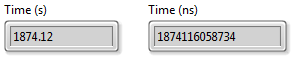
\includegraphics[width=0.35\linewidth]{IMG/ch5/latch_tests/fig20.PNG}
	\caption{Timestamp measured after 30 min = 1800 s\\initial time $\approx$ 74.1 s.}
	\label{fig:timestamptest}
\end{figure}

\subsection{Rate measurements for multiple channels}\label{RateMeasurements}
\noindent In this section it will be shown the results of the rate measurements. In order to do a rate measurement two instants (states) were saved using the latch system at two different addresses. Using formula \ref{eq:rate} the rate was calculated for each channel and the plotted:
\begin{equation}\label{eq:rate}
	Rate\:=\: \frac{\Delta N_i}{\Delta T}
\end{equation}
\noindent with $N_i$ the number of counts at the $i^{th}$ channel and $\Delta T$ the difference between the two saved timestamps.
In figures \ref{fig:latchrate10} \ref{fig:latchrate50} \ref{fig:latchrate75} \ref{fig:latchrate110} it can be seen a graph for each impulsed frequency. On the X axis there is the channel number and on the Y axis there is the calculated rate in kHz. It can be observed that the even channels that are counting have a measured rate that is perfectly compatible with the theoretical one.
The biggest discrepancy appears in figure \ref{fig:50khz} where against a sent frequency of 50~kHz, one of 49.9998~kHz is measured. The difference is 0.2~Hz, which is less than the 1\% clinical tolerance. However much more measurements and test are needed in order to calculate the precision of those numbers.
It is noteworthy the behaviour of \textit{ch23}. This is an odd channel, it does not receive any test pulse, however it is counting. This is due to cross-talk effects.
From the figures shown earlier it emerges that this behaviour becomes less and less pronounced at higher rate.
If in the first case (figures \ref{fig:latchrate10} and \ref{fig:10khz}) the measured rate is almost 100\% of the sent one, in the next tests this value drops to:
63.1\% for the 50~kHz case (figures \ref{fig:latchrate50} and \ref{fig:50khz}),
55,8\% for the 75~kHz case (figures \ref{fig:latchrate75} and \ref{fig:75khz}) and
42.5\% for the 110~kHz case (figures \ref{fig:latchrate110} and \ref{fig:110khz}).
\newline
\noindent These measurements where made by pressing in the proper order the three buttons of the \textit{Manual latch controls} tab of figure \ref{fig:newlabviewpanel}.
This process is not yet automated, thus there is no consistency between the time difference ($\Delta T$) of the two latched states.
The next important step is to create an automated rate calculation logic in LabVIEW which can autonomously send the commands to the FPGA with a setted, precise and configurable delay (integration time).
\begin{figure}[H]
	\centering
	\begin{minipage}{0.24\textwidth}
		\centering
		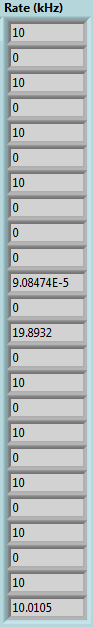
\includegraphics[width=.7\linewidth]{IMG/ch5/latch_tests/fig16}
		\caption{Pulsed rate=\\10~kHz.}
		\label{fig:10khz}
	\end{minipage}
	\begin{minipage}{0.24\textwidth}
		\centering
		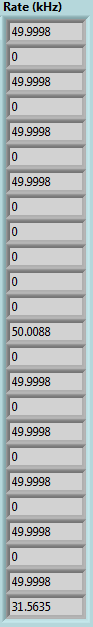
\includegraphics[width=.7\linewidth]{IMG/ch5/latch_tests/fig17}
		\caption{Pulsed rate=\\50~kHz.}
		\label{fig:50khz}
	\end{minipage}
	\begin{minipage}{0.24\textwidth}
		\centering
		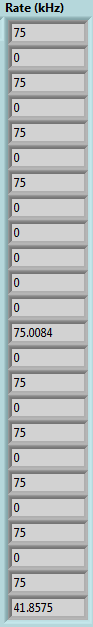
\includegraphics[width=.7\linewidth]{IMG/ch5/latch_tests/fig18}
		\caption{Pulsed rate=\\75~kHz.}
		\label{fig:75khz}
	\end{minipage}
	\begin{minipage}{0.24\textwidth}
		\centering
		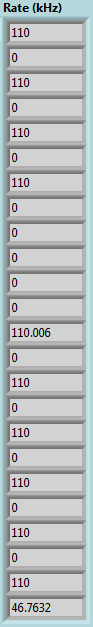
\includegraphics[width=.7\linewidth]{IMG/ch5/latch_tests/fig19}
		\caption{Pulsed rate=\\110~kHz.}
		\label{fig:110khz}
	\end{minipage}
\end{figure}
%%% [!htpb]
\begin{figure}[H]
	\centering
	\begin{minipage}{0.49\textwidth}
		\centering
		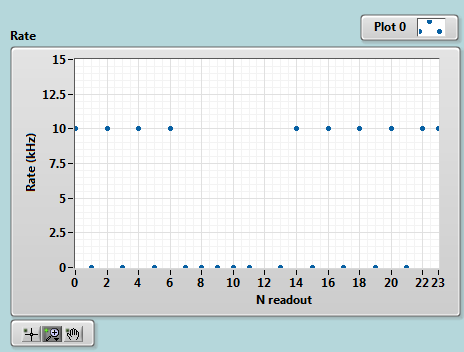
\includegraphics[width=.95\linewidth]{IMG/ch5/latch_tests/fig3.PNG}
		\caption{Latch Rate calculation at 10~kHz impulse rate.}
		\label{fig:latchrate10}
	\end{minipage}%
	\begin{minipage}{0.49\textwidth}
		\centering
		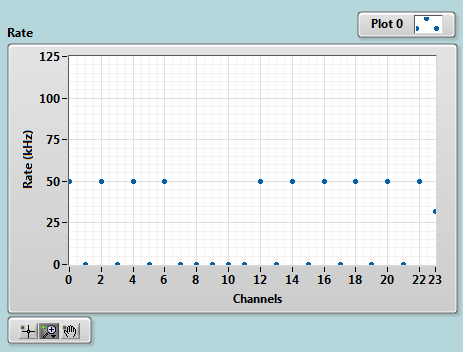
\includegraphics[width=.95\linewidth]{IMG/ch5/latch_tests/fig5.PNG}
		\caption{Latch Rate calculation at 50~kHz impulse rate.}
		\label{fig:latchrate50}
	\end{minipage}
\end{figure}
\begin{figure}[H]
	\centering
	\begin{minipage}{0.49\textwidth}
		\centering
		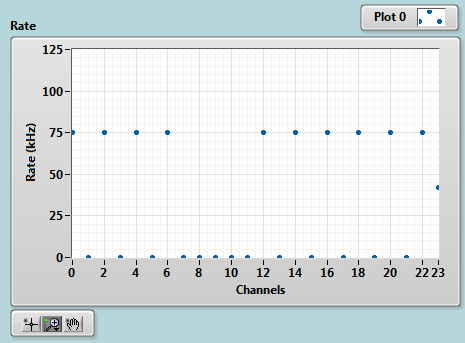
\includegraphics[width=.95\linewidth]{IMG/ch5/latch_tests/fig9.PNG}
		\caption{Latch Rate calculation at 75~kHz impulse rate.}
		\label{fig:latchrate75}
	\end{minipage}%
	\begin{minipage}{0.49\textwidth}
		\centering
		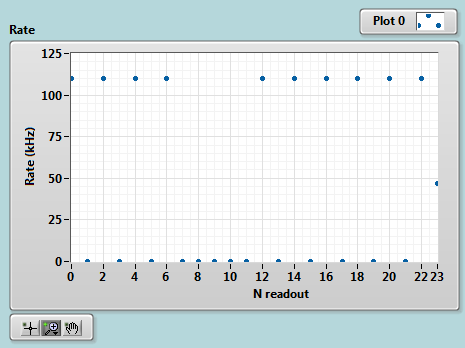
\includegraphics[width=.95\linewidth]{IMG/ch5/latch_tests/fig12.PNG}
		\caption{Latch Rate calculation at 110~kHz impulse rate.}
		\label{fig:latchrate110}
	\end{minipage}
\end{figure}

\subsection{Rate measurement for single channel}\label{RateMeasurements2}
\noindent In order to study the new rate measurement accuracy and to compare it with the previous method the automated LabVIEW rate calculation logic was implemented and the following tests were performed.
The fast pulse generator was configured at 1~MHz and the rate was measured 999 times with four different integration times (100~ms, 200~ms, 300~ms and 500~ms). This was performed with the "old" method, that uses the computer CPU time to calculate the rate (in figures \ref{fig:CPU-time-rate-1MHz-100ms}, \ref{fig:CPU-time-rate-1MHz-200ms}, \ref{fig:CPU-time-rate-1MHz-300ms} and \ref{fig:CPU-time-rate-1MHz-500ms}), and with the new timestamp method (in figures \ref{fig:FPGA-time-rate-1MHz-100ms}, \ref{fig:FPGA-time-rate-1MHz-200ms}, \ref{fig:FPGA-time-rate-1MHz-300ms} and \ref{fig:FPGA-time-rate-1MHz-500ms}).
For each measurement a histogram was generated and a Gaussian fit was performed in order to quantify the standard deviation~$\sigma$. 
The results are divided for each integration time.
To be noted that with the "CPU" method the lowest possible integration time is 100~ms due to the used LabVIEW panel.
A lower $\sigma$ means that the measurements, considering equal integration times, are less spread apart, thus more precise.
All measurements were performed on data from \textit{ch16}.

\subsubsection{1 MHz, 100 ms}
\begin{figure}[H]
	\centering
	\begin{minipage}{0.49\textwidth}
		\centering
		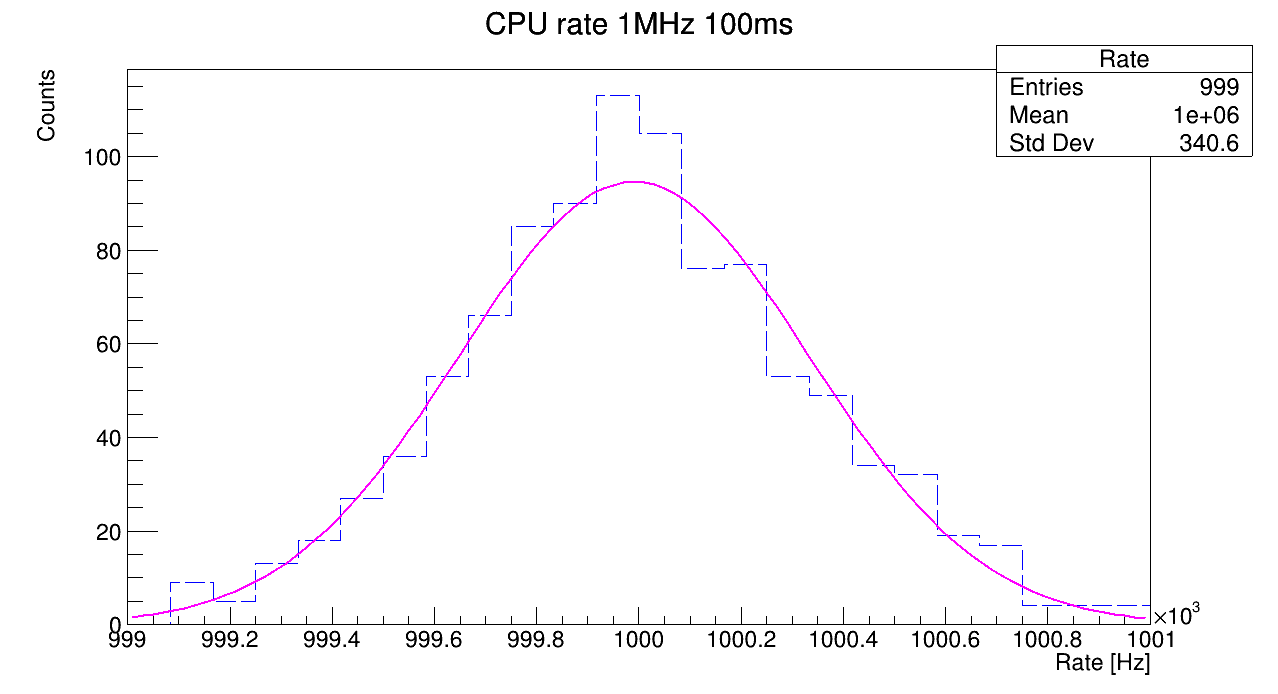
\includegraphics[width=.95\linewidth]{IMG/ch5/RateMeasures/CPU-time-rate-1MHz-100ms}
		\caption{1 MHz pulsed rate\\100 ms integration time\\CPU time method.}
		\label{fig:CPU-time-rate-1MHz-100ms}
	\end{minipage}%
	\begin{minipage}{0.49\textwidth}
		\centering
		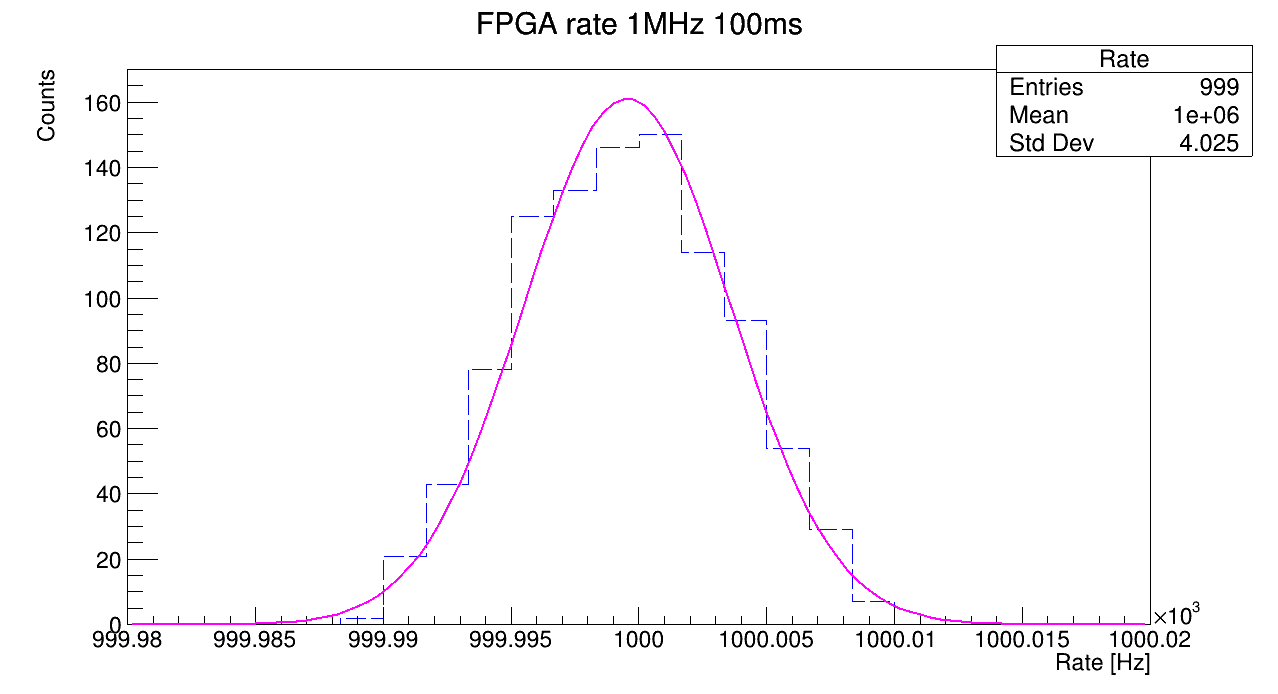
\includegraphics[width=.95\linewidth]{IMG/ch5/RateMeasures/FPGA-time-rate-1MHz-100ms}
		\caption{1 MHz pulsed rate\\100 ms integration time\\FPGA time method.}
		\label{fig:FPGA-time-rate-1MHz-100ms}
	\end{minipage}
\end{figure}
\noindent CPU method $\rightarrow$ measured $\sigma_{CPU}$ = 340.6 Hz
\newline
FPGA method $\rightarrow$ measured $\sigma_{FPGA}$ = 4.0 Hz
\begin{equation}
	\frac{\sigma_{CPU}}{\sigma_{FPGA}} = 85.2
\end{equation}


\subsubsection{1 MHz, 200 ms}
\begin{figure}[H]
	\centering
	\begin{minipage}{0.49\textwidth}
		\centering
		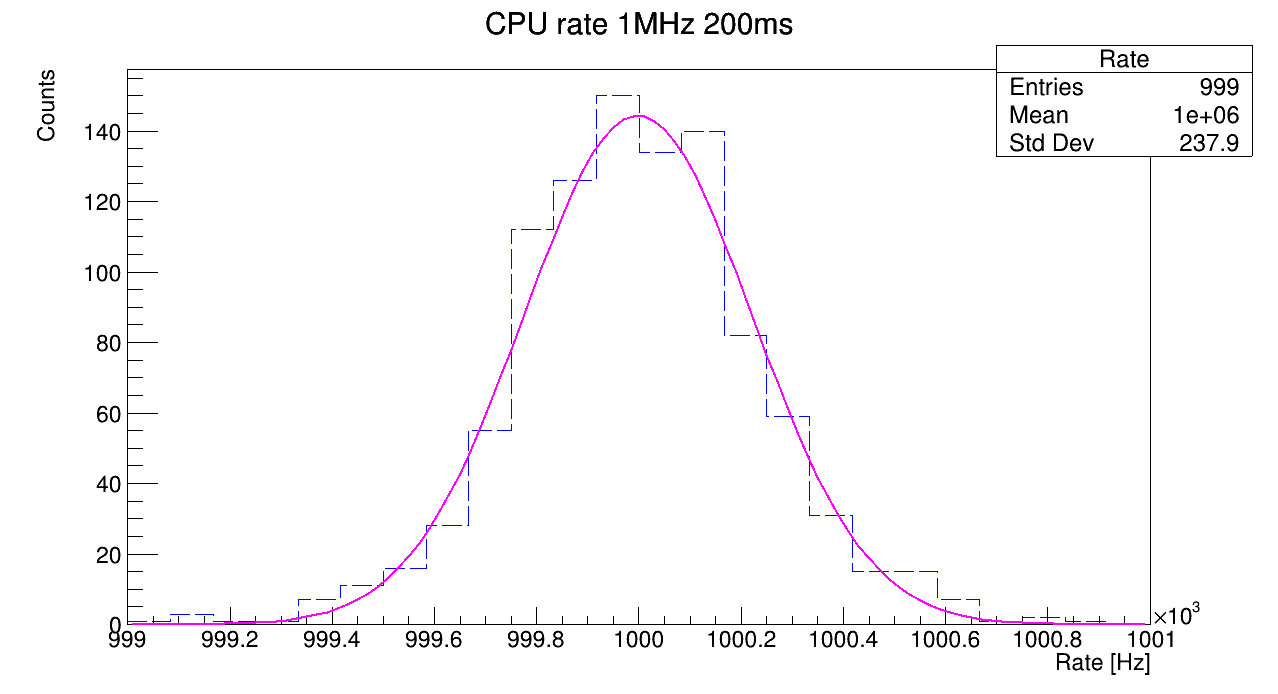
\includegraphics[width=.99\linewidth]{IMG/ch5/RateMeasures/CPU-time-rate-1MHz-200ms}
		\caption{1 MHz pulsed rate\\200 ms integration time\\CPU time method.}
		\label{fig:CPU-time-rate-1MHz-200ms}
	\end{minipage}%
	\begin{minipage}{0.49\textwidth}
		\centering
		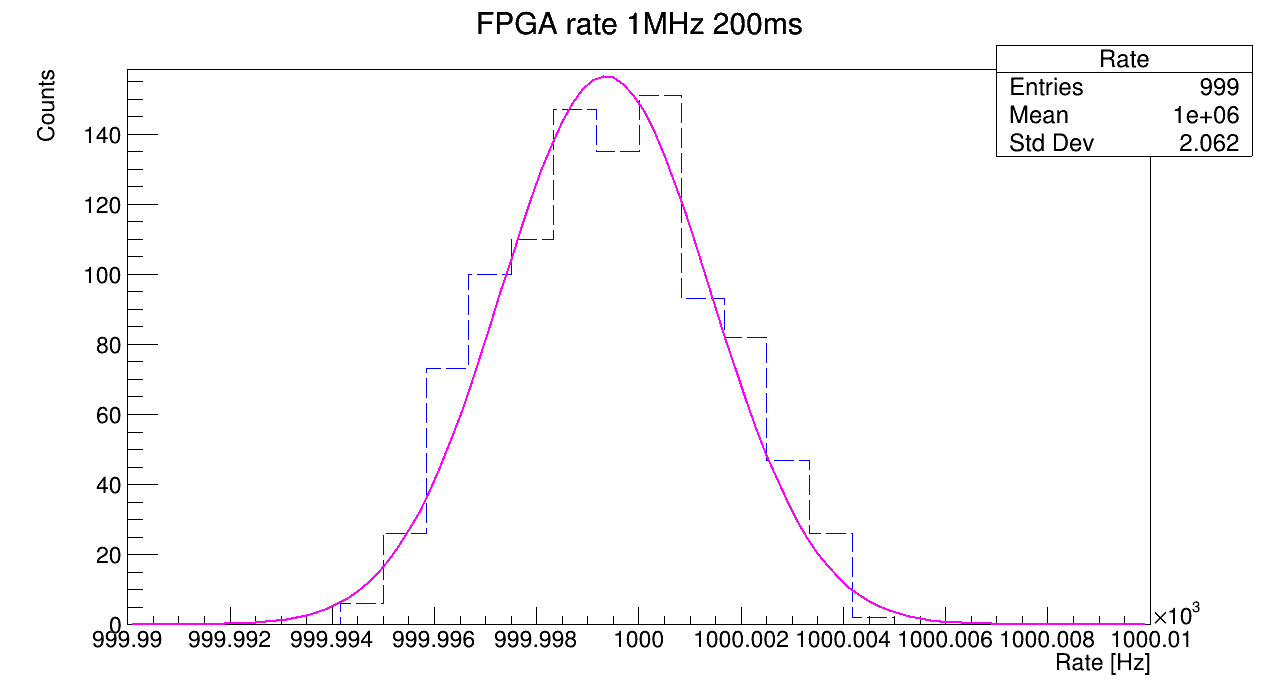
\includegraphics[width=.99\linewidth]{IMG/ch5/RateMeasures/FPGA-time-rate-1MHz-200ms}
		\caption{1 MHz pulsed rate\\200 ms integration time\\FPGA time method.}
		\label{fig:FPGA-time-rate-1MHz-200ms}
	\end{minipage}
\end{figure}
\noindent CPU method $\rightarrow$ measured $\sigma_{CPU}$ = 237.9 Hz
\newline
FPGA method $\rightarrow$ measured $\sigma_{FPGA}$ = 2.1 Hz
\begin{equation}
	\frac{\sigma_{CPU}}{\sigma_{FPGA}} = 113.3
\end{equation}

\subsubsection{1 MHz, 300 ms}
\begin{figure}[H]
	\centering
	\begin{minipage}{0.49\textwidth}
		\centering
		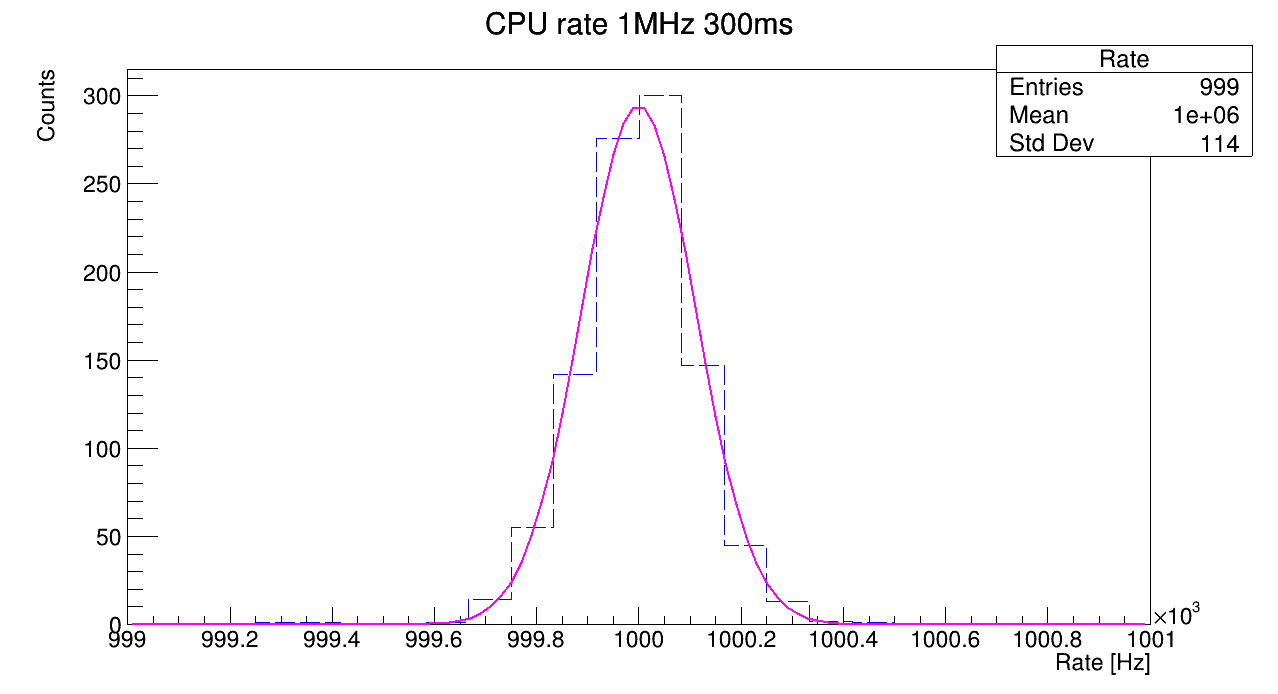
\includegraphics[width=.99\linewidth]{IMG/ch5/RateMeasures/CPU-time-rate-1MHz-300ms}
		\caption{1 MHz pulsed rate\\300 ms integration time\\CPU time method.}
		\label{fig:CPU-time-rate-1MHz-300ms}
	\end{minipage}%
	\begin{minipage}{0.49\textwidth}
		\centering
		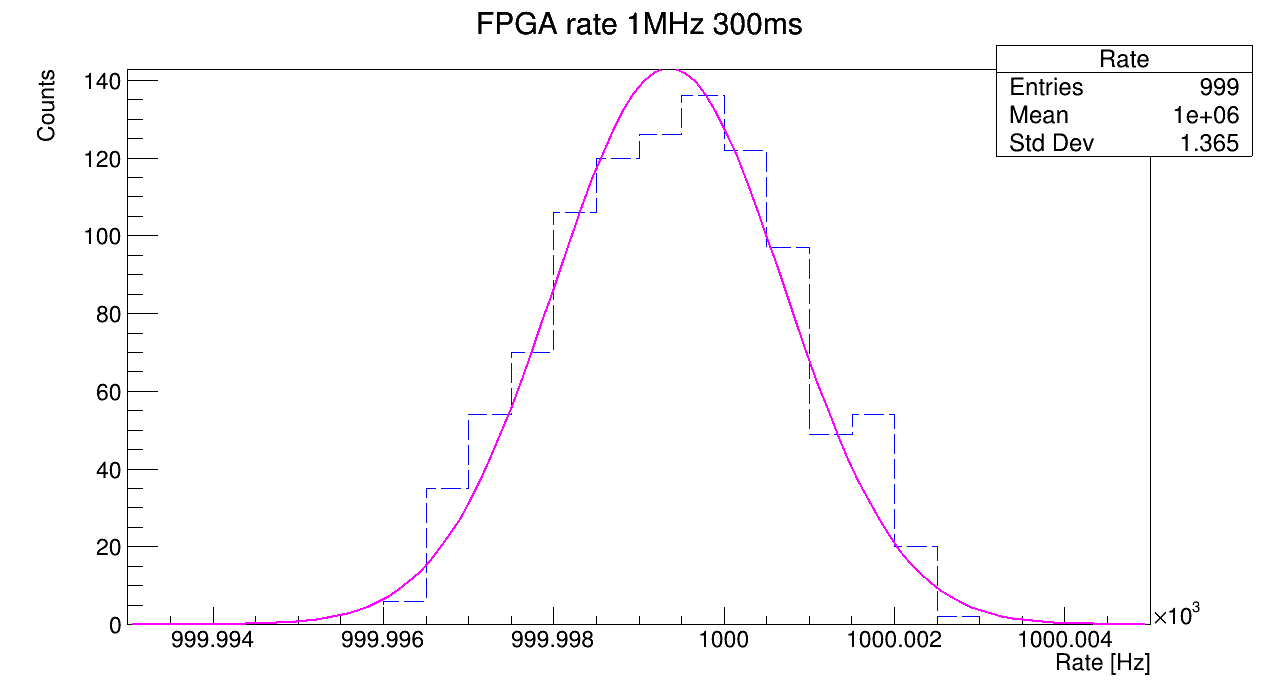
\includegraphics[width=.99\linewidth]{IMG/ch5/RateMeasures/FPGA-time-rate-1MHz-300ms}
		\caption{1 MHz pulsed rate\\300 ms integration time\\FPGA time method.}
		\label{fig:FPGA-time-rate-1MHz-300ms}
	\end{minipage}
\end{figure}
\noindent CPU method $\rightarrow$ measured $\sigma_{CPU}$ = 114.0 Hz
\newline
FPGA method $\rightarrow$ measured $\sigma_{FPGA}$ = 1.4 Hz
\begin{equation}
	\frac{\sigma_{CPU}}{\sigma_{FPGA}} = 81.4
\end{equation}

\subsubsection{1 MHz, 500 ms}
\begin{figure}[H]
	\centering
	\begin{minipage}{0.49\textwidth}
		\centering
		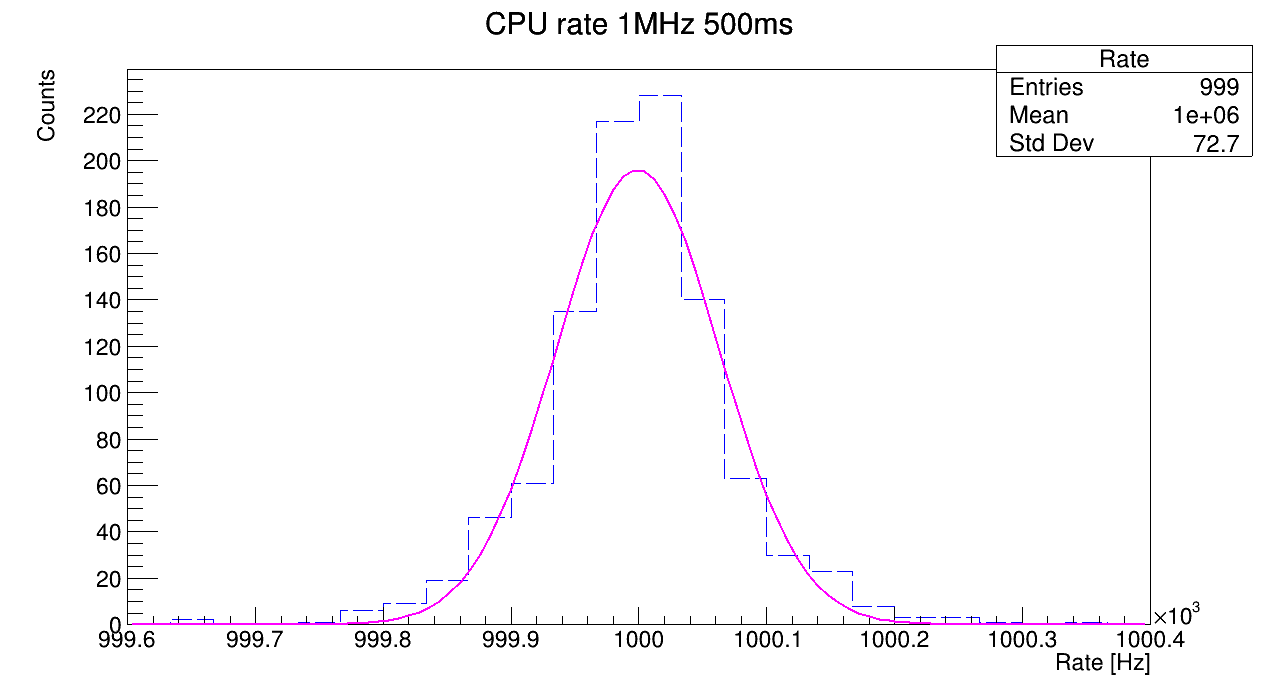
\includegraphics[width=.99\linewidth]{IMG/ch5/RateMeasures/CPU-time-rate-1MHz-500ms}
		\caption{1 MHz pulsed rate\\500 ms integration time\\CPU time method.}
		\label{fig:CPU-time-rate-1MHz-500ms}
	\end{minipage}%
	\begin{minipage}{0.49\textwidth}
		\centering
		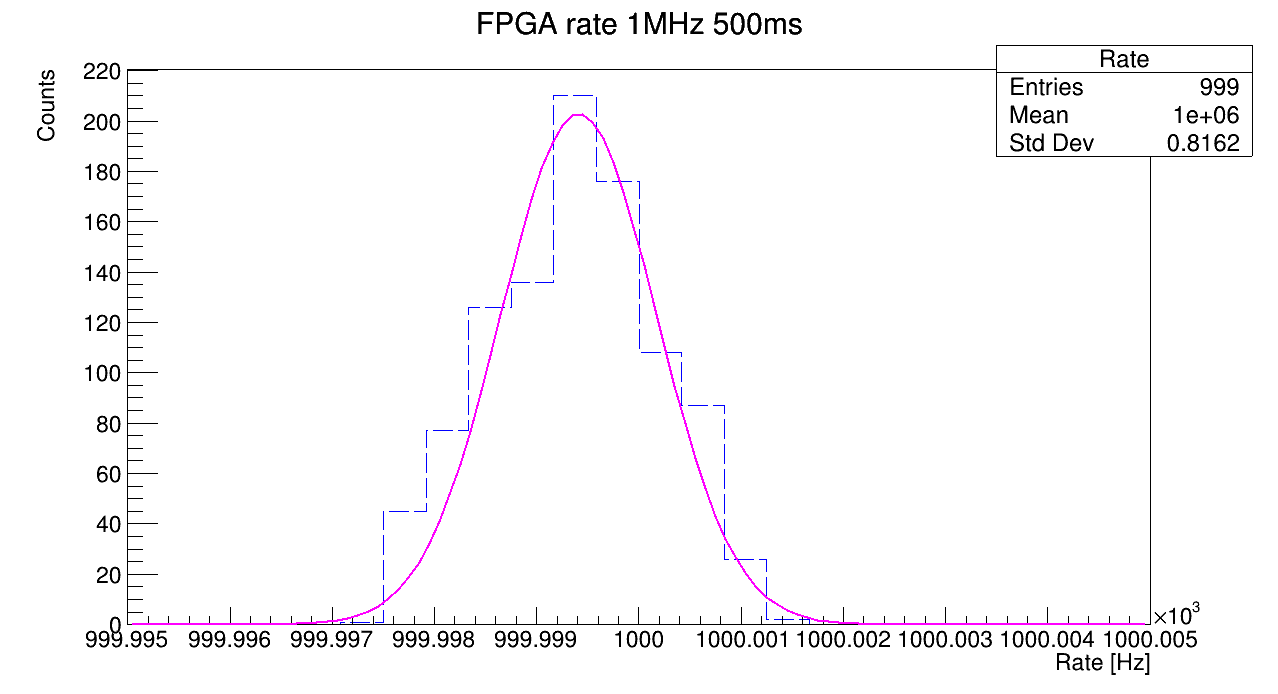
\includegraphics[width=.99\linewidth]{IMG/ch5/RateMeasures/FPGA-time-rate-1MHz-500ms}
		\caption{1 MHz pulsed rate\\500 ms integration time\\FPGA time method.}
		\label{fig:FPGA-time-rate-1MHz-500ms}
	\end{minipage}
\end{figure}
\noindent CPU method $\rightarrow$ measured $\sigma_{CPU}$ = 72.7 Hz
\newline
FPGA method $\rightarrow$ measured $\sigma_{FPGA}$ = 0.8 Hz
\begin{equation}
	\frac{\sigma_{CPU}}{\sigma_{FPGA}} = 90.9
\end{equation}
\newline
\noindent \textbf{The average gain in standard deviation is 92.7.}
\newline
This means that the new way to measure the rate is almost 90 times more precise than the old one.

\subsubsection{1 MHz, 50 ms and 1 ms}
\noindent With the new method it is possible to overcome the 100~ms integration time limit. Thus two more test have been performed, one with 50~ms integration time in figure \ref{fig:FPGA-time-rate-1MHz-50ms} and one with 1~ms in figure \ref{fig:FPGA-time-rate-1MHz-1ms}.
For the 50~ms case $\sigma_{FPGA}$~=~8.0~Hz, this is still almost 10 times lower than the $\sigma_{CPU}$ at 500~ms (72.7~Hz).   
\begin{figure}[H]
	\centering
	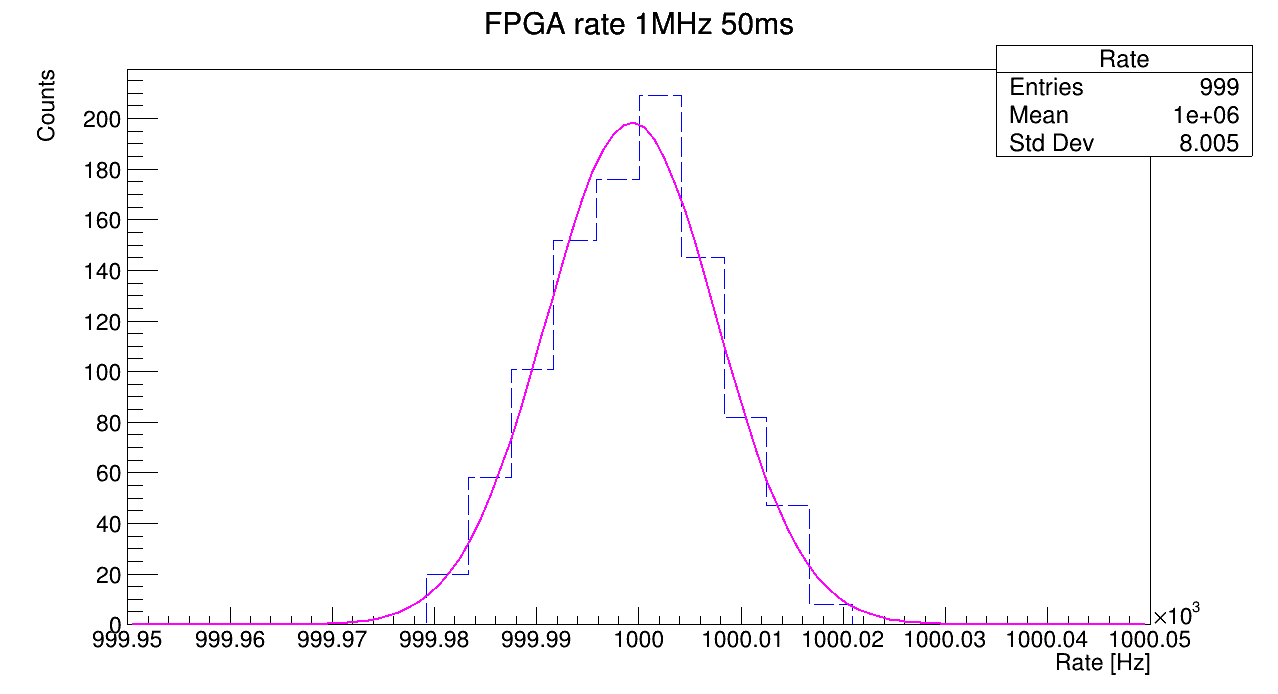
\includegraphics[width=0.95\linewidth]{IMG/ch5/RateMeasures/FPGA-time-rate-1MHz-50ms}
	\caption{1 MHz pulsed rate\\50 ms integration time\\FPGA time method.}
	\label{fig:FPGA-time-rate-1MHz-50ms}
\end{figure}
\noindent Lowering the integration time even more, down to 1~ms, makes the measurement less accurate ($\sigma_{FPGA}$~=~408.7~Hz), however the error is still less than 1\% which is perfectly compatible with the required clinical precision.
\begin{figure}[H]
	\centering
	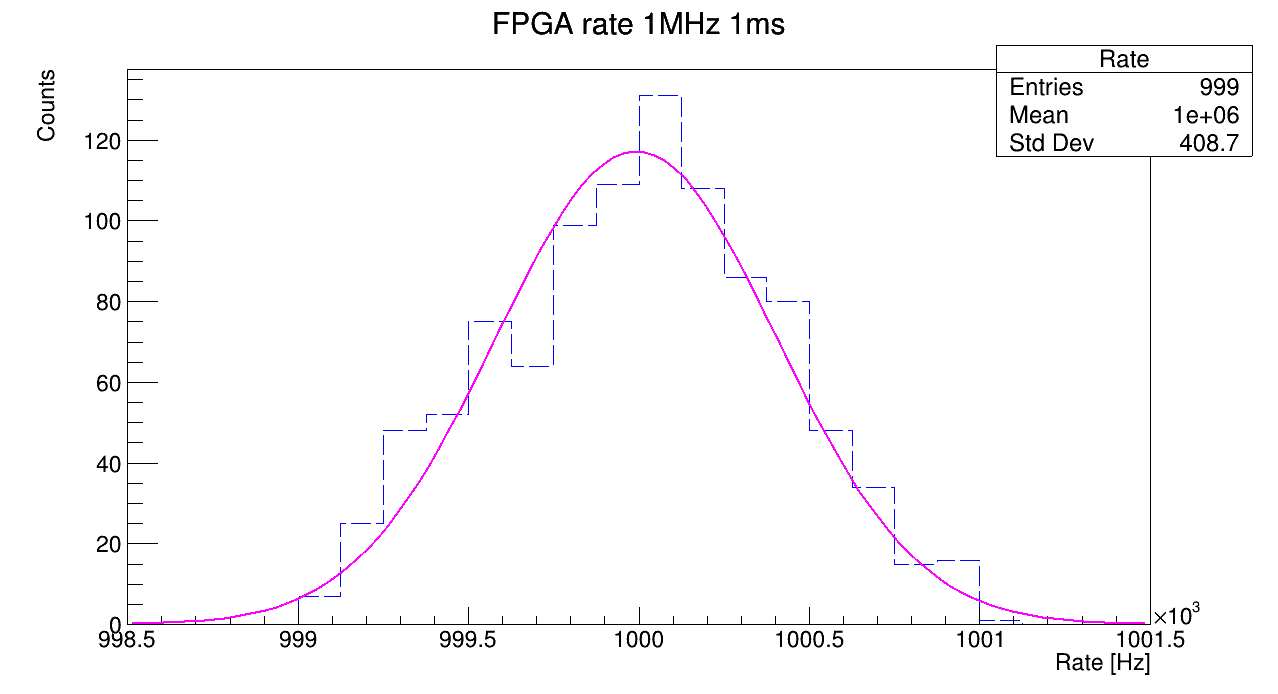
\includegraphics[width=0.95\linewidth]{IMG/ch5/RateMeasures/FPGA-time-rate-1MHz-1ms}
	\caption{1 MHz pulsed rate\\1 ms integration time\\FPGA time method.}
	\label{fig:FPGA-time-rate-1MHz-1ms}
\end{figure}

\subsubsection{Improvement visualization}
\noindent In order to better visualize the accuracy improvement the following plot have been generated. In red it can bee seen the histogram of the CPU calculated rate, while in black it can be seen the FPGA calculated rate. The comparison has been made using the 100~ms integration time case with 1~MHz pulsed rate. The improvement is remarkable and can be seen in figure \ref{fig:FPGA_and_CPU_rate_1MHz_100ms}. 
\begin{figure}[H]
	\centering
	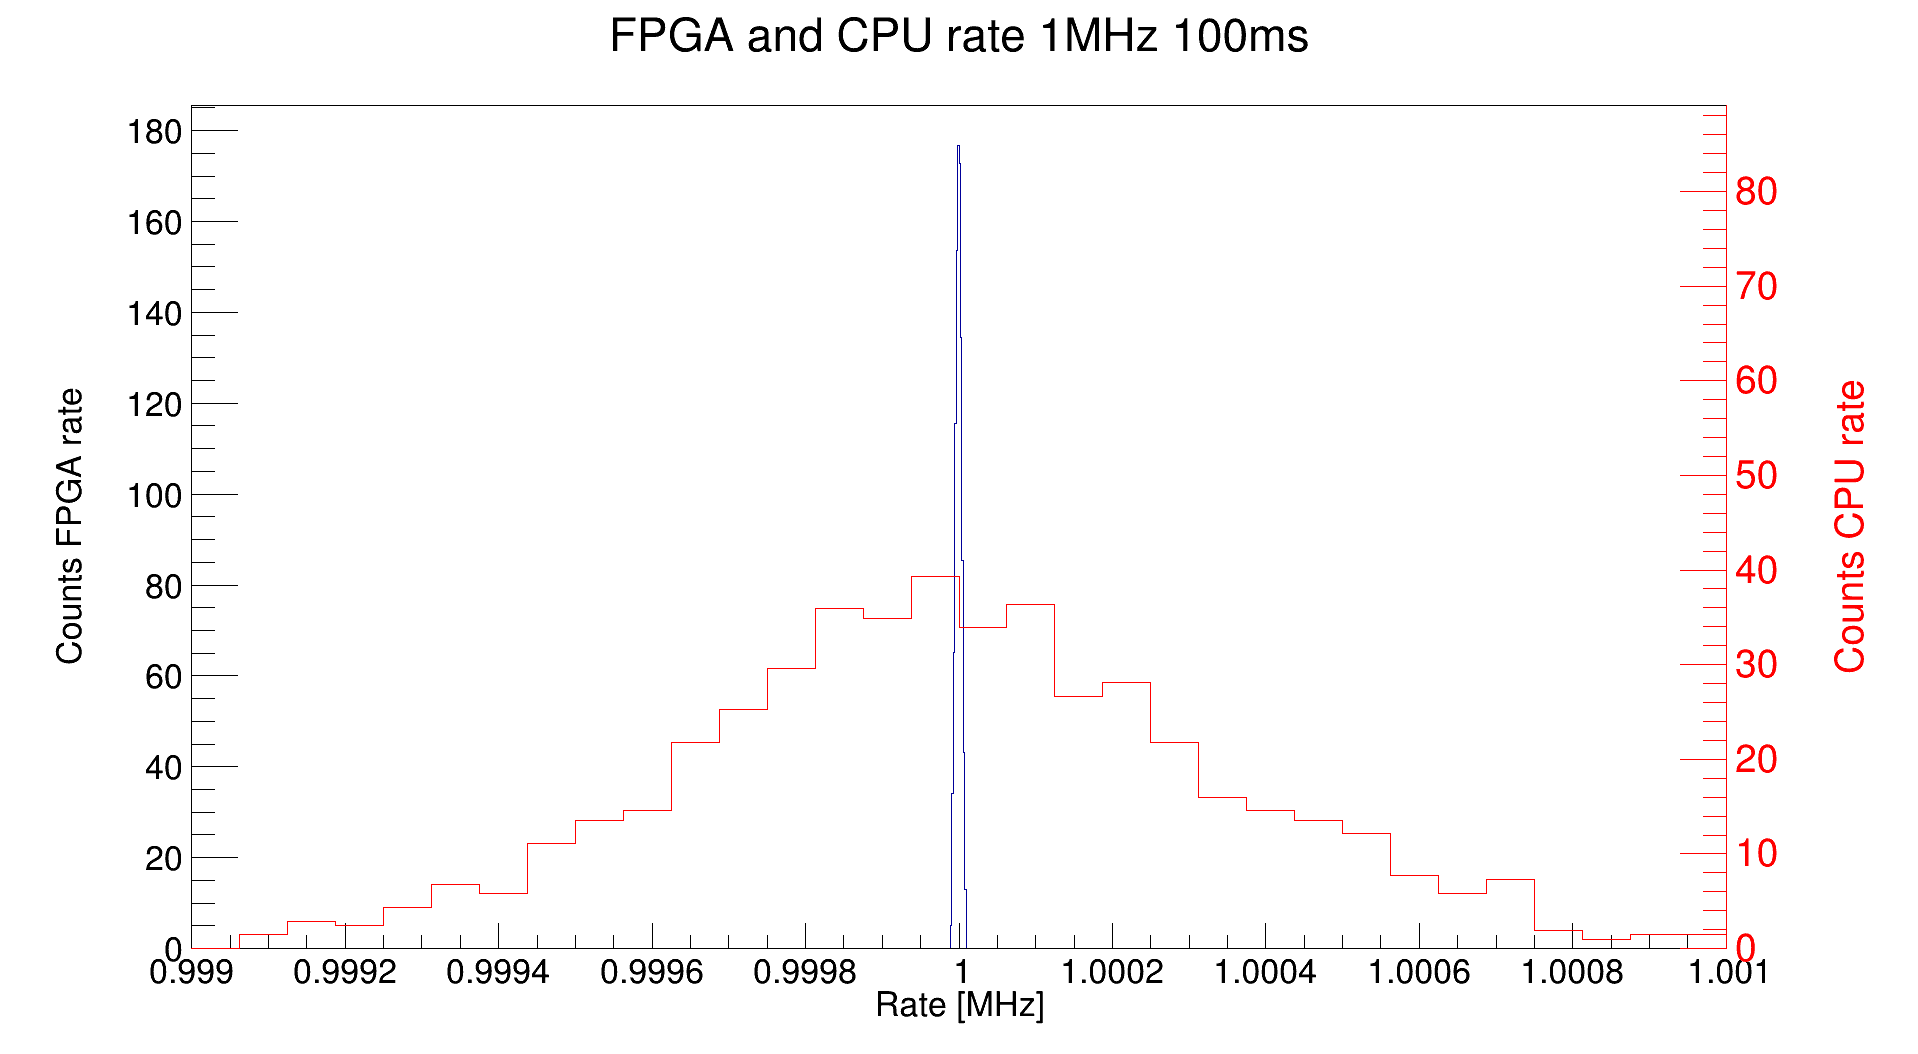
\includegraphics[width=0.95\linewidth]{IMG/ch5/RateMeasures/FPGA_and_CPU_rate_1MHz_100ms}
	\caption{1 MHz pulsed rate; 100~ms integration time\\FPGA time method in black, CPU time method in red.}
	\label{fig:FPGA_and_CPU_rate_1MHz_100ms}
\end{figure}










